\chapter{Diskussion}
\label{ch:diskussion}

\section{\norm{Bėide} als Quantor}
\label{sec:beidequant}

In beiden Datenserien, dem \tit{Corpus der altdeutschen Originalurkunden}
(\CAO{}) und der \tit{Kaiserchronik} (\KC{}), ist der direkte Bezug zwischen
der Kombination von zwei Substantiven\is{Substantiv} oder eines Substantivs mit
einem \isi{Personalpronomen} als \isi{Controller} in Bezug auf ein
\norm{bėide}-\isi{Target} selten belegt. Nichtsdestoweniger zeigen sich
dieselben Muster, die auch für den häufiger belegten Kontext mit einem Pronomen
zwischen \isi{Controller} und Target beobachtet wurden. Im Fall der \KC{} sind
im gesammelten Material keine Belege für den unbelebten\is{Inanimata} Bezug
vorhanden, weswegen das \CAO{}-Material hier allein betrachtet werden muss. Der
Quantor \norm{al} `alle' \autocite[vgl.][606--621]{ksw2} kommt in der \KC{} im
relevanten Kontext nahezu ausschließlich mit Bezug auf einzelne Substan\-tive
im Plural vor, bietet also auch kaum Vergleichspunkte. Die Daten für die
Kombination von maskulin-männlichen und feminin-weiblichen
Controllern\is{Controller} stützen sich ebenfalls maßgeblich auf das \CAO{}, da
die \KC{} aufgrund ihres Inhalts kaum Belege dazu hergibt.

Die Beobachtungen der Belegauswertung zur Kongruenzform von Targets\is{Target}
in Abhängigkeit von den kombinierten Personenmerkmalen\is{Personenmerkmal}
ihrer \isi{Controller} in \sectref{sec:caotargpers} und
\sectref{sec:kctargpers} lassen sich wie in \tabref{tab:caokcrules_1} und
\ref{tab:caokcrules_2} zusammenfassen. Auf die Reihenfolge\is{Abfolge} der
Referenten kommt es dabei nicht an, ebenso wenig auf den
Wortformenabstand\is{Distanz!lineare} zwischen \isi{Controller} und Target. Bei
den Urkunden\is{Urkunde} hatte sich gezeigt, dass ein Vokal nach der
Flexionsendung \norm{-e/-iu} keine auffällig neutrali\-sie\-rende Wirkung auf
diese hat, sodass etwa ausschließlich \norm{e} geschrieben würde. Die
entsprechenden Belege wurden hier daher mitgezählt.

\begin{table}
\caption{belebte Controller\is{Controller}}
\begin{tabular}{l l r r}
\lsptoprule

Sexus
	& Kongruenzform
	& \norm{bėide}
	& \norm{bėidiu}
	\\

\midrule

$\SM + \SM$
	& \textsc{m+f}, selten \textsc{n}
	& 31
	& 3
	\\

$\SF + \SF$
	& \textsc{m+f}
	& 7
	& %
	\\

$\SM + \SF$
	& \textsc{n}, häufiger \textsc{m+f}
	& 19
	& 57
	\\

$\SF + \SX$
	& \textsc{n}, daneben \textsc{m+f}
	& 1
	& 1
	\\

\lspbottomrule
\end{tabular}
\label{tab:caokcrules_1}
\end{table}
	
\begin{table}
\caption{unbelebte Controller}
\begin{tabular}{l l r r}
\lsptoprule

Genus
	& Kongruenzform
	& \norm{bėide}
	& \norm{bėidiu}
	\\

\midrule

$\MascI + \MascI$
	& \textsc{n}, selten \textsc{m+f}
	& 2
	& 5
	\\

$\NeutI + \NeutI$
	& \textsc{n}
	& %
	& 24
	\\

$\MascI + \FemI$
	& \textsc{n}
	& %
	& 4
	\\

$\MascI + \NeutI$
	& \textsc{n}
	& %
	& 4
	\\

$\FemI + \NeutI$
	& \textsc{n}
	& %
	& 1
	\\

\lspbottomrule
\end{tabular}
\label{tab:caokcrules_2}
\end{table}

Die generelle Beobachtung, dass zwei belebte\is{Animata} \isi{Controller} mit
unterschiedlichem Geschlecht \isi{Gender Resolution} erfahren und durch ein
Neutrum aufgenommen werden, hat sich weitestgehend auch im untersuchten
Material bestätigt\is{Validierung}.%
%
	\footnote{Auch im 20.~Jahrhundert\il{Neuhochdeutsch} finden sich noch
		Belege wie der folgende, in dem mit
		individualisierendem\is{Individualisierbarkeit} Bezug auf Anatol Stiller
		(\MascM) und seine Geliebte Sabine (\FemF) statt dem heute geläufigen
		Maskulinum oder einer gendersensiblen\is{Gender} Form wie \fw{jede*r}
		das Neutrum steht: \textquote{Stumm saßen \emph{sie}
		\textins{\textsc{3pl\subMF.nom}} auf der Erde, zwei Ehebrecher in
		zärtlicher Verflechtung ihrer Hände, \emph{jedes}
		\textins{jeder-\textsc{nom.sg.n\subMF.st}} mit einem Halm zwischen den
		sorgenvoll-ver\-bis\-senen Lippen \textelp{}} (Max Frisch:
		\tit{Stiller}; \cite[332--333]{frisch:stiller}; Hervorhebung und
		Annotation CB; vgl.~auch \cite[188]{dal2014} sowie Beispiel
		\ref{ex:m+f_si_beidiu_float}, Seite \pageref{ex:m+f_si_beidiu_float}).
		% = Heft 6, Ende 3. Abschnitt
	}
%
Bezüglich verschiedener Erklärungs\-ansätze für dieses Phänomen übt
\citet[213--221]{askedal1973} ausführlich Kritik an der
junggrammatischen\is{Junggrammatik} Hypothese, dass \isi{Gender Resolution}
durch das Neutrum im Germanischen\il{Germanisch} auf den
historischen\is{Diachronie} Zusammenfall des Nom./Akk.\ \isi{Dual} M.\ mit dem
Nom./Akk.~Pl.~N.\ durch die Laut\-entwicklung vom
Indogermanischen\il{Indogermanisch} zum Germanischen\il{Germanisch}
zurückzuführen sei: \foreignblockcquote{english}[196]{ringe2017}{The PIE
nom.-acc.\ dual\is{Dual} masculine of o-stems (probably the default\is{Default}
stem-class of nouns) ended in *-oh₁; the nom.-acc.\ plural neuter of o-stems
ended in *-ah₂. The regular phonological development of those two endings was
as follows: *-oh₁ > *-ō \textelp{} > *-ā > *-ō \textelp{}; *-ah₂ > *-ā
\textelp{} > *-ā > *-ō \textelp{}. It can be seen that the two endings merged
in *-ā during the development of PGmc.}

Auch \citeauthor{behaghel1928} führt diese These an,\is{Junggrammatik} vermerkt
jedoch, dass \blockcquote[40]{behaghel1928}{W.~Schulze \textelp{} nach
mündlicher Mitteilung Bedenken\is{Vorbehalt} gegen diese Erklärung} habe, ohne
auf dessen Argument einzugehen. Auch \citet[157]{hock2008},
\citet[196]{ringe2017} und \citet[104]{miller2019} führen die Dual-Hypothese
als Ursprung für die Setzung des Neutrums als Resolutionsgenus\is{Gender
Resolution} an. Da der \isi{Dual} als Flexionskategorie jedoch bereits im
Althochdeutschen\il{Althochdeutsch} keine Rolle mehr spielt, ist es fraglich,
die lautgeschichtliche Entwicklung als alleinige Begründung für die im
Mittel\-hoch\-deutschen\il{Mittelhochdeutsch} existierende Regel zu bemühen,
zumal diese nicht begründet, warum die Setzung des Neutrums als
Resolutionsgenus\is{Gender Resolution} über Jahrhunderte Bestand hatte, auch
wenn der \isi{Dual}-Zusammenfall als Anstoß für die \isi{Grammatikalisierung}
des Neutrums als Resolutionsgenus\is{Gender Resolution} bei Personen gewirkt
haben mag.

\citet{askedal1973} sieht die Motivation dafür in einer auf
Personenmerkmalen\is{Personenmerkmal} basierenden, syntaktischen Regel und ist
in dieser Hinsicht ein Vorläufer von \citet{corbett1983} und
\citet{wechslerzlatic2003}. In Bezug auf \posscite[246--247]{delbrueck1900}
Annahme, dass die Setzung des Neutrums bei kombiniertem Personenbezug im
Germanischen\il{Germanisch} eine Ausweitung der für \isi{Inanimata} bereits im
Indogermanischen\il{Indogermanisch} geltenden Regel darstellt
\autocite[vgl.~auch][156--157]{hock2008}, geht er davon aus, dass die von
\citet[28]{behaghel1928} und \citet[188]{dal2014} als \textquote{von alters
her} geltend und \textquote{ursprünglich} charaktersierte Regel als eine
\blockcquote[15]{askedal1973}{irgendwann im Urgermanischen
eintretende\textdel{} Veränderung einer aus dem Idg.\ stammenden
Kongruenzregel} zu verstehen ist.

Beim Bezug von \norm{bėide} auf einzelne Substantive\is{Substantiv} im Plural
ist im Gegensatz zum kombinierten Bezug im ausgewerteten Material formale
Kongruenz die Regel. Doch auch hier steht zumindest in Einzelfällen
unregelmäßig\is{Ausnahme} eine neutrale Form (\norm{bėidiu}), wo eine maskuline
(\norm{bėide}) zu erwarten wäre. Dies ist der Fall bei je einem Vorkommen der
sehr eindeutig Männer denotierenden\is{Denotation} Maskulina \norm{rihtǟre}
`Richter' und \norm{hērre} `Herr' \REF{ex:richtherriu3}.

\begin{exe}
\ex \label{ex:richtherriu3}
	\begin{xlist}
	\ex \gll Die rihtær ſprachen beideu {dar zuͦ} \\
			die Richter[\textsc{nom.pl.\MascM}] sprachen
				beide-\textsc{nom.pl.\NeutM.st} dazu \\
		\trans `Die Richter äußerten sich beide dazu'
			(%
				B1:~28ra,8; vgl.~abweichend
				\KC:~V.~10090;
				\cite[267]{schroeder1895}% 1140 mit Parallelstelle in H
			)
		\label{ex:richtherriu3_1}

	\ex \gll Die herren baten ir ſa \\
			Die Herren[\textsc{nom.pl.\MascM}] baten ihr alsbald \\
	\sn \gll Beideu beſvnder \\
			beide-\textsc{nom.pl.\NeutM.st} einzeln \\
		\trans `Die Herren hielten alsbald jeweils beide um ihre Hand an.'
			(%
				B1:~31va,48--49; vgl.
				\KC:~V.~11385--11386;
				\cite[289]{schroeder1895}% 1112x
			)
		\label{ex:richtherriu3_2}
	\end{xlist}
\end{exe}

Umgekehrt enthält das Material zum \CAO{} einen Beleg, bei dem in
Bezug auf das un\-belebte Neutrum \lit{gvt} `Gut' die maskulin-feminine
Form \lit{baide} statt der erwarteten neutralen Form vom Typ \norm{bėidiu}
auftritt \REF{ex:1584_gut2}.

\begin{exe}
\ex\label{ex:1584_gut2}
	\gll ſo ſint baide gvt / dev wiſe / vn̄ freioltzmoſen /
			ledichleichen / dez gotzhauſ datze phaffenwerd \\
		so sind beide-\textsc{nom.pl.m+f?\subI.st} Gut[\textsc{nom.pl.\NeutI}]
			{} die Wiese {} und Freiolzmosen {} frei {} des Gotteshaus da=zu
			Pfaffenwerde \\
	\trans `so stehen beide Güter, die Wiese und Freiolzmosen, dem Gotteshaus
		in Pfaffenwerde zur freien Verfügung'
		\parencites(Nr.~1584, Kl.~Herrenchiemsee, Kr.~Rosenheim, 1292)[727,26--27]{cao2}
\end{exe}

Als Erklärungsansatz für diese und andere Belege bieten sich die Arbeiten von
\citet[171--195]{wechslerzlatic2003} beziehungsweise \citet{wechsler2009} an.
Sie behandeln darin das Thema \isi{Genus}\-kongruenz im Rahmen der
LFG\is{Lexical-functional Grammar}
\autocites(vgl.~\sectref{sec:lfgkongr}){bresnanetal2016} und stellen die
Hierarchie zur \isi{Genuszuweisung} in \REF{ex:gendasshier} auf (\fw{gender
assignment hierarchy}; \cites[584]{wechsler2009}[195]{wechslerzlatic2003}).

\begin{exe}
\ex\label{ex:gendasshier}
	\begin{enumerate}[noitemsep]
		\item inhärentes grammatisches Geschlecht (wenn die
			NP\is{Nominalphrase} einen \isi{Kopf} mit einem Genuswert\is{Genus}
			hat). Andernfalls:
		\item semantisches Geschlecht (wenn sich die \isi{Denotation} der NP
			innerhalb der \isi{Domäne} des semantischen Klassifikationssystems
			befindet). Andernfalls:
		\item Regel zur Ableitung des \isi{Genus} kumulierter
			unbelebter\is{Inanimata} Diskursreferenten.
	\end{enumerate}
\end{exe}

Zu beachten ist, dass gerade die erste Regel zum inhärenten grammatischen
Geschlecht beim kombinierten Bezug eines Targets\is{Target} auf zwei
\isi{Controller} nicht zutrifft. Die einzelnen \isi{Controller} besitzen zwar
jeweils für sich Personenmerkmale\is{Personenmerkmal}, von denen Geschlecht --
grammatisches (\isi{Genus}) oder semantisches (\isi{Sexus}) -- eines ist. Für
die Kombination der Nominalphrasen\is{Nominalphrase} lässt sich jedoch kein
einzelner, eindeutiger Phrasenkopf\is{Kopf} (\xhead{N})
identifizieren,\is{Ambiguität} mit dessen \isi{Genusmerkmal} problemlos
kongruiert werden kann, was in \figref{fig:npconstit} anhand einer
Koordinations\-konstruktion\is{Koordination} verdeutlicht wird.

\begin{figure}
\begin{forest} shorter edges, narrower nodes,
	[NP
		[\xbar{N}
			[\xhead{N}
				[A]
			]
		]
	]
\end{forest}
\hspace{2em}
\begin{forest} shorter edges, narrower nodes,
	[NP
		[\xbar{N}
			[\xhead{N}
				[A]
			]
			[Conj
				[und]
			]
			[\xhead{N}
				[B]
			]
		]
	]
\end{forest}
\caption{Einfacher und komplexer Phrasenkopf einer NP}
\label{fig:npconstit}
\end{figure}

Als Folge ergibt sich, dass die zweite Regel angewandt wird und das \isi{Genus}
zugunsten semantischer Eigenschaften aufgelöst wird, wenn möglich. Bei den
Animata\is{Animata} vollzieht sich \isi{Gender Resolution} laut
\citet[573]{wechsler2009} mittels der Bedeutung (\isi{Sexus}) der koordinierten
NP\is{Nominalphrase} und nicht der Form (\isi{Genus}) der
NP-Konjunkte.\is{Koordination}
%
	% \footnote{\foreignblockcquote{english}[573]{wechsler2009}{\textins*{G}ender
	% 	resolution for animates proceeds by consulting the meaning (\q{natural
	% 	gender}, i.e.\ sex) of the coordinate NP and not the form
	% 	(\q{grammatical gender}) of the conjunct NPs}.% }
%
Wie in \sectref{sec:erwkonjbegr} erörtert, gilt dies im Kontext von
\norm{bėide} nicht nur für syntaktisch koordinierte\is{Koordination} Nominale,
sondern auch für syntaktisch voneinander unabhängige Nominalphasen, auf die
sich ein \isi{Target} aber gleichzeitig bezieht.

\subsection{Direkter Bezug zwischen Controller und Target}
\label{subsec:beid2coord}
\is{Controller|(}
\is{Target|(}

In \REF{ex:gendassgmt1_txt} wird ein Beispiel für den Fall gegeben, in dem das
Target \lit{pediv} `beide' mit nur einem nominalen Controller \lit{Jnſidel}
`Siegel' kongruiert. Es handelt sich dabei um ein unbelebtes\is{Inanimata}
\isi{Substantiv}, daher definiert \lit{Jnſidel} sein \isi{Genusmerkmal} über
das \isi{Lexikon}: Es ist ein Neutrum%
% (\figref{fig:gendassgmt1_morphlex})
. Das Target \lit{pediv} kongruiert mit seinem Controller in den formalen
Kategorien Kasus, \isi{Genus} und \isi{Numerus}. Da nur ein Controller
involviert ist, kann dessen \isi{Genusmerkmal} einfach auf Kompatibilität
abgeprüft werden: Das Target verlangt gemäß seiner Wortform vom Typ
\norm{bėidiu} ein Neutrum; sein Controller \lit{Jnſidel} `Siegel' bietet gemäß
seines Lexikoneintrags\is{Lexikon} das Neutrum als \isi{Genusmerkmal}.
Kongruenz kommt also zustande (\sectref{sec:lfgkongr}).

\begin{exe}
\ex \label{ex:gendassgmt1_txt}
	\gll vnſriv pediv Jnſidel \\
		unser-\textsc{acc.pl.\NeutI.st} beide-\textsc{acc.pl.\NeutI.st}
			Siegel[\textsc{acc.pl.\NeutI}] \\
	\trans `unsere beiden Siegel'
		\parencites(Nr.~3224~A, Freising, 1299)[400,12--13]{cao4}
\end{exe}

% \begin{figure}
% \begin{tabular}[t]{@{} l @{\hspace{2em}} c @{\hspace{2em}} l}
% \norm{insigel}
% 	&	N
% 	&	\begin{tabular}[t]{@{} l l l @{}}
% 			\ups{pred}	& =	& `Siegel' \\
% 			\ups{anim}	& = & $-$ \\
% 			\ups{gend}	& =	& \textsc{n} \\
% 			\ups{pers}	& =	& 3 \\
% 		\end{tabular}
% \end{tabular}
% \caption{Morpholexikalische Definition von \norm{insigel} `Siegel'}
% \label{fig:gendassgmt1_morphlex}
% \end{figure}

Dasselbe gilt auch, wenn das Target innerhalb des gleichen Satzes in
\isi{Distanzstellung} zu seinem Controller steht, also ein
\isi{Floating Quantifier} vorliegt (\sectref{sec:floatquant}). In
\REF{ex:gendassgmt2} bezieht sich das Target \lit{baide} auf den Controller
\lit{rihtære} `Richter', wobei der Quantor hinter dem finiten Verb im
\isi{Mittelfeld} und damit getrennt von dem \isi{Substantiv} steht, das er
modifiziert.\is{Distanzstellung} Der Zusammenhang zwischen beiden aufeinander
bezogenen Teilen wird durch Kongruenz angezeigt.

\begin{exe}
\ex \label{ex:gendassgmt2}
	\gll Die richtare ſprachen dar beide zuͦ. \\
		die Richter[\textsc{nom.pl\subM}] sprachen da
		beide-\textsc{nom.pl\subM.st} zu \\
	\trans `Die Richter äußerten sich beide dazu'
		(%
			H:~60vb,28; vgl.~abweichend
			\KC:~V.~10090;
			\cite[267]{schroeder1895}%
		)
\end{exe}

Gerade in diesem Kontext wäre die Untersuchung von Hybrid Nouns wie \norm{wīp}
`Frau (\NeutF)' interessant,\is{Desiderat} da dadurch Aufschluss darüber
erlangt würde, ob beim direkten Bezug auf ein einzelnes Plural-\isi{Substantiv}
formale\is{Kongruenz!formale} oder semantische
Kongruenz\is{Kongruenz!semantische} eintritt. Entsprechende Belege sind aber
weder im exzerptierten \CAO{}- noch im \KC{}-Material vorhanden. Auch eine
Suche im \REM{} nach Formen von \norm{bėide} in direkter Abhängigkeit von einem
belebten\is{Animata} Plural-Substantiv war nicht erfolgreich.

Angemerkt sei, dass die Stelle in \REF{ex:gendassgmt2} zwischen den Fassungen
variiert. \citet[244]{myers2013} übersetzt sinngemäß: \textquote{but the judges
said to both the Jews and the heathens} (fehlt bei \cite[177--178]{mayer1874}).
Der Wortlaut der Stelle in den verschiedenen Handschriften wird in
\REF{ex:gendassgmt2_var} zitiert.

\begin{exe}
\ex \label{ex:gendassgmt2_var}
	\begin{tabular}[t]{
	@{}
	>{\itshape}l @{~}
	>{\itshape}l @{~}
	>{\itshape}l @{~}
	>{\itshape}l @{~}
	>{\itshape}l @{~}
	>{\itshape}l @{~}
	>{\itshape}l
	l
	@{}
}
di
	& rihtrære
	& ſprachen
	& der
	& baide
	& %
	& zuͦ
	& (A1:~44ra,29--30)
	\\

Die
	& richtare
	& ſprachen
	& dar
	& beide
	& %
	& zuͦ.
	& (H:~60vb,28)
	\\

Divͤ
	& richter
	& ſprachen
	& in
	& peid
	& %
	& zuͤ.
	& (W:~68va,13--14)
	\\

Die
	& rihtær
	& ſprachen
	& %
	& beideu
	& dar
	& zuͦ
	& (B1:~28ra,8)
	\\

Die
	& rihtære
	& ſprachen
	& %
	& %
	& dar
	& zv
	& (VB:~48va,23)
	\\

Die
	& richtær
	& ſprachen
	& %
	& %
	& da
	& zvͦ.
	& (C1:~53ra,29)
	\\
\end{tabular}
\end{exe}

Eine Interpretation mit partitivem \norm{dęr} in \norm{dęr bėide} `beiden
(\textsc{dat.pl}) von ihnen' erlaubt allein A1
\autocite[vgl.][s.\,v.~\textit{zuo sprëchen}]{lexer:mhdhwb}, allerdings wäre
als Dativform regelmäßig \norm{bėiden} zu erwarten \autocite[182]{ksw2}. Mit
Ausnahme\is{Ausnahme} von B1 enthalten nur die Handschriften der Rezension~A
\norm{bėide}, das in H und B1 auf \norm{rihtǟre} `Richter' bezogen zu sein
scheint, möglicherweise auch in W. Jedenfalls ist \norm{bėidiu} in B1 keine
typische Dativform, die analog zu der Stelle in A1 und möglicherweise in W als
Ziel von \norm{zue spręchen} `zusprechen' dienen könnte. Die anderen B- und
C-Fassungen unterscheiden sich im Wortlaut ansonsten nicht von VB.

\is{Target|)}

\subsubsection{Belebte kombinierte Controller}
\label{subsubsec:x+x_dir_anim}
\is{Animata|(}

\citet[182--183]{wechslerzlatic2003} und \citet[576]{wechsler2009}
argumentieren hinsichtlich des Bezugs eines Targets\is{Target} auf eine
Kombination von Controllern, dass eine koordinierte\is{Koordination}
NP\is{Nominalphrase} kein Kopf\-nomen\is{Substantiv}\is{Kopf} beinhalte,
insofern bei koordinierten nominalen Konjunkten die übliche klare
Projektionslinie von genau einem N-\isi{Kopf} zur NP-Ebene fehle
\autocites[183, Fußnote 85]{wechslerzlatic2003}[585, Fußnote 7]{wechsler2009}.
Der Knoten \q{NP} enthält bei der \isi{Koordination} statt einem Unterknoten
drei (siehe
\figref{fig:npconstit}).%
%
	\footnote{Aus Sicht der Government-and-Binding-Theorie\is{Government and
	Binding} beziehungsweise des \isi{Minimalismus} gehen beispielsweise
	\textcites{johannessen1998}{johannessen2005} und \citet{shen2019} davon
	aus, dass es eine funktionale ConjP oder \&P mit der \isi{Konjunktion} als
	\isi{Kopf} gibt \autocite[dagegen aber][]{borsley2005}. Die
	LFG\is{Lexical-functional Grammar} geht dagegen davon aus, dass die
	Konjunkte nicht gestuft, sondern gleichwertig nebeneinander stehen
	\autocites[vgl.~z.\,B.][]{peterson2004}{sadlernordlinger2006}.}
%
Dies habe zur Folge, dass bei belebten Konjunkten semantische Resolution
eintrete \autocites[183]{wechslerzlatic2003}[576]{wechsler2009}. Bei
unbelebten\is{Inanimata} Konjunkten tritt stattdessen gemäß Regel 3 in
\REF{ex:gendasshier} eine formale Regel zur Auflösung\is{Gender Resolution} in
Kraft, da hier keine semantischen
Geschlechtsmerkmale\is{Sexusmerkmal}\is{Merkmale!semantische} geltend gemacht
werden können, sondern nur formale.\is{Merkmale!grammatische}

Ein Beispiel für \isi{Gender Resolution} im Bezug auf belebte Controller wird
in \REF{ex:gendres2} gegeben. Hier treten \lit{Rvͦdiger} `Rüdiger (\MascM)' und
\lit{ſin hovſfrowe} `seine Ehefrau (\FemF)' als kombinierte Controller auf, die
durch das Target\is{Target} \lit{bediv} (\NeutMF) gemeinsam aufgenommen werden.
Gemischt männliche und weibliche Referenz wird mit dem Neutrum als derjenigen
Option markiert, die weder männliche noch weibliche Personen bezeichnet. Dass
semantische Kriterien im Spiel sind, wird darin sichtbar, dass die
\norm{e}-Form formal gleichermaßen maskuline und feminine Referenten
bezeichnet. Dies wird deutlich in der Analyse der einzelnen Pluralcontroller in
\chapref{ch:caoanalyse} und \ref{ch:kcanalyse} für die
oberdeutschen\il{Oberdeutsch} Urkunden und diejenigen \KC{}-Handschriften, bei
denen im Plural das Neutrum noch klar vom Maskulinum-Femininum unterschieden
wird. Nach rein formalen Kriterien wäre also keine \isi{Gender Resolution}
notwendig.

\begin{exe}
\ex \label{ex:gendres2}
		\gll swenne aber her Rvͦdiger vnd ſin
			hovſfrowe bediv niht enſint \\
		so=wenn aber Herr Rüdiger[\textsc{nom.sg.\MascM}] und sein
			Ehefrau[\textsc{nom.sg.\FemF}] beide-\textsc{nom.pl.\NeutMF.st}
			nicht \textsc{neg}=sind \\
		\trans `Wenn aber Herr Rüdiger und seine Ehefrau
			beide nicht \textins{mehr} sind'
			\parencites(Nr.~3262, Regensburg, 1299)[425,13--14]{cao4}
\end{exe}

\citeauthor{wechsler2009} (\citeyear{wechsler2009}: 576;
\cite[vgl.~auch][182]{wechslerzlatic2003}) erklärt weiter, dass \isi{Sexus}
eine distributive Eigenschaft sei und schlussfolgert, dass die Menge der
distributiven Eigenschaften einer Gruppe gleich der Schnittmenge der
distributiven Eigenschaften jedes Gruppenmitglieds ist
(\sectref{sec:indexconcord}).\is{Concord}
%
	% \footnote{\foreigntextquote{english}[{\cites[576]{wechsler2009}[vgl.][182]{wechslerzlatic2003}}]{%
	% 	Sex is a distributive property \textelp{}. As a rule the set of
	% 	distributive properties of a group is just the intersection of the sets
	% 	of distributive properties of each of the group's members}. }
%
\isi{Gender Resolution} tritt also dem Modell zufolge immer dann ein, wenn
semantische Geschlechtsmerkmale\is{Sexusmerkmal}\is{Merkmale!semantische}
(\isi{Sexus}) keine Schnittmenge bilden können wie in \figref{fig:sexintersect}
schematisch dargestellt.

\begin{figure}
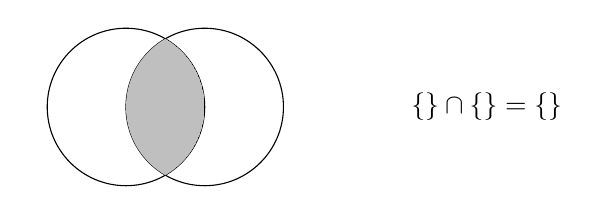
\begin{tikzpicture}[
	baseline=(current bounding box.north),
	set/.style = {
		circle,
		draw,
		minimum size = 2cm
	}
]
\node[set, label={180:\SM}] (M1) at (0,0) {};
\node[set, label={  0:\SM}] (M2) at (1,0) {};
\begin{scope}
	\clip (0,0) circle(1cm);
	\clip (1,0) circle(1cm);
	\fill[lightgray](0,0) circle(1cm);
\end{scope}
\node at (.5,0) {\SM};
\node[anchor=west,align=left] at (3.5,0) {$\{\SM\} \cap \{\SM\} = \{\SM\}$};
\end{tikzpicture}\medskip

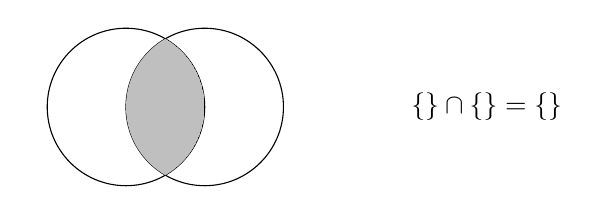
\begin{tikzpicture}[
	baseline=(current bounding box.north),
	set/.style = {
		circle,
		draw,
		minimum size = 2cm
	}
]
\node[set, label={180:\SF}] (F1) at (0,0) {};
\node[set, label={  0:\SF}] (F2) at (1,0) {};
\begin{scope}
	\clip (0,0) circle(1cm);
	\clip (1,0) circle(1cm);
	\fill[lightgray](0,0) circle(1cm);
\end{scope}
\node at (.5,0) {\SF};
\node[anchor=west,align=left] at (3.5,0) {$\{\SF\} \cap \{\SF\} = \{\SF\}$};
\end{tikzpicture}\medskip

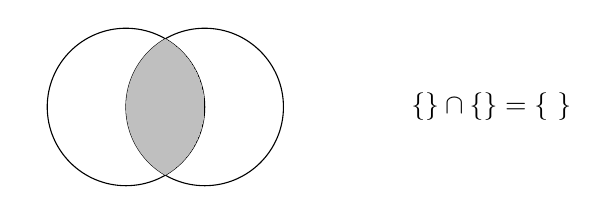
\begin{tikzpicture}[
	baseline=(current bounding box.north),
	set/.style = {
		circle,
		draw,
		minimum size = 2cm
	}
]
\node[set, label={180:\SM}] (M) at (0,0) {};
\node[set, label={  0:\SF}] (F) at (1,0) {};
\begin{scope}
	\clip (0,0) circle(1cm);
	\clip (1,0) circle(1cm);
	\fill[lightgray](0,0) circle(1cm);
\end{scope}
\node at (.5,0) {};
\node[anchor=west,align=left] at (3.5,0) {$\{\SM\} \cap \{\SF\} = \{\ \}$};
\end{tikzpicture}
\caption{Kombination der Sexus-Merkmale belebter Controller}
\label{fig:sexintersect}
\end{figure}

Die Menge an Belegen für den direkten Bezug zwischen Controller und
\isi{Target} ist sowohl im \CAO{} als auch in der \KC{} sehr klein
(vgl.~\sectref{subsubsec:perscombsgnp}, \sectref{subsubsec:conomctrlpers}). Ein
Beispiel für die Kombination zweier weiblicher Controller mit direktem Bezug
zum Target kann im gesammelten Belegmaterial nicht gefunden werden.%
%
	\footnote{Kursorische Suchen im \CAO{} sowie im \REM{} nach kombinierten
	belebten Feminina, die direkt durch eine adjektivisch flektierende Wortart
	modifiziert werden, waren ergebnislos.}
%
Das zweite Diagramm in \figref{fig:sexintersect} ist daher eine begründete
Annahme, die sich auf Belege mit indirektem Bezug zwischen Controller und
Target stützt (siehe~\sectref{subsec:beid2p2coordrefl}). Das Beispiel in
\REF{ex:dietwill3} zeigt die Kombi\-nation zweier männlicher Personen; ein
Beispiel für die Kombination einer männlichen und einer weiblichen Person wurde
bereits in \REF{ex:gendres2} gegeben.

\begin{exe}
\ex\label{ex:dietwill3}
		\gll Willehalm vnd Dietreich. \\
			Willehalm[\textsc{nom.sg.\MascM}] und Dietrich[\textsc{nom.sg.\MascM}] \\
	\sn \gll wurden baíde da erſlagen. \\
			wurden beide-\textsc{nom.pl.\MascM.st} da erschlagen \\
		\trans `Willehalm und Dietrich wurden beide dort erschlagen.'
			(%
				C1:~83vb,36--37; vgl.
				K:~95vb,12--13%
			)
\end{exe}

\citet[576]{wechsler2009} und \citet[182]{wechslerzlatic2003} folgend lässt
sich die Situation auch für das Mittelhochdeutsche\il{Mittelhochdeutsch} so
erklären, dass zwei Typen von Genera\is{Genus} unterschieden werden können:
einerseits Genera\is{Genus} mit semantischen Korrelaten wie das Maskulinum und
das Femininum und andererseits Genera\is{Genus} ohne semantische Korrelate wie
das Neutrum.

\is{Animata|)}

\subsubsection{Unbelebte kombinierte Controller}
\label{subsubsec:x+x_dir_inan}
\is{Inanimata|(}

Der einzige Beleg im gesammelten Material für den direkten Bezug des
Targets\is{Target} auf zwei unbelebte Controller ist der in
\REF{ex:hofzehntbeidiu} zitierte, der mit \lit{hof} `Hof' und \lit{zehenden}
`Zehnten' zwei Maskulina enthält. Diese werden durch pronominal verwendetes
\lit{beidev} aufgenommen, der Form nach ein Neutrum. Dasselbe Muster zeigt sich
beim indirekten Bezug zwischen Controllern und Target noch weitere vier Male im
\CAO{}. Die Frage ist, inwiefern dies Regel oder Ausnahme\is{Ausnahme}
darstellt. In regelmäßigen Fällen ist zu erwarten, dass zwei maskulin-unbelebte
Controller ein ebenfalls maskulines Target produzieren.

\begin{exe}
\ex\label{ex:hofzehntbeidiu}
	% Text auskommentiert, weil sonst Hurenkind resultiert :(
	\gll minen hof \textelp{} verkaufft han mit dem
			zehenden \textelp{}, beidev vnuerſchaidenlichen
			% fvͤr reht aigen
			\\
			meinen Hof[\textsc{acc.sg.\MascI}] {} verkauft habe mit dem
			Zehnt-\textsc{dat.sg.\MascI} {} beide-\textsc{acc.pl.\NeutI.st}
			gleichermaßen
			% für rechtmäßig Eigentum
			\\
	\trans `meinen Hof verkauft habe mit dem Zehnten \textelp{}, beide
		gleichermaßen%
		% zum rechtmäßigen Eigentum
		'
		\parencites(Nr.~N~241, Augsburg, 1283)[195,37--39]{cao5}
\end{exe}

Die Resolutionsform von Inanimata wird gemäß dem Modell von
\citet{wechsler2009} durch die Schnittmenge zwischen den grammatischen
Genera\is{Genus} der Konjunkte und deren Schnittmenge mit der Menge der
formalen Korrelate der semantischen Geschlechter ($\SM \sim \textsc{m}$; $\SF
\sim \textsc{f}$) gebildet. Da das Neutrum die Resolutionsform darstellt, ist
es als leere Menge definiert
\autocites[vgl.][576--578]{wechsler2009}[184--186]{wechslerzlatic2003}. Damit
ergibt sich für das Mittelhochdeutsche\il{Mittelhochdeutsch} ein ähnliches
System wie im Färöischen\il{Färöisch} oder im Isländischen\il{Isländisch}
\autocites[225--226]{thrainsson2004}{wechsler2009}, wie in \figref{fig:iclgr}
gezeigt. Anders als das Mittelhochdeutsche\il{Mittelhochdeutsch} besitzen diese
im Nom.~Pl. (Isländisch\il{Isländisch} auch im Akk.~Pl.) der starken
\isi{Adjektivdeklination} unterschiedliche Endungen für die einzelnen
Genera\is{Genus}, siehe \tabref{tab:faerislmhdadj}.
% %
% 	\footnote{Für das Färöische\il{Färöisch} bzw.\ das
% 		Isländische\il{Isländisch} geben \citet[100--101]{thrainsson2004} und
% 		\citet[84--90]{kress1982} an:
% 		\fw{-ir}/\fw{-ar}/-Ø (Nom.~Pl.~M./F./N.) bzw.\ \fw{-a(r)}/\fw{-ar}/-Ø
% 		(Akk.~Pl.~M./F./N.). Dem gegenüber steht mhd.-obd.
% 		\fw{-e}/\fw{-e}/\fw{-iu} (Nom./Akk.~Pl.~M./F./N.;
% 		\cite[182--183]{ksw2}); siehe auch \tabref{tab:faerislmhdadj}.%
% 	}

\begin{figure}
	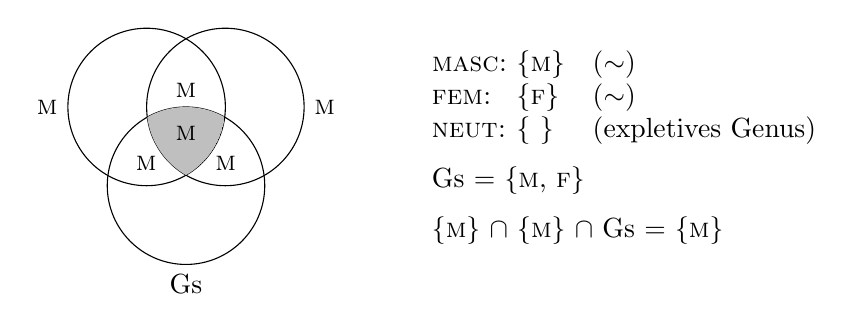
\begin{tikzpicture}[
		baseline=(current bounding box.north),
		set/.style = {
			circle,
			draw,
			minimum size = 2cm
		}
	]

	\node[set, label={180:\textsc{m}}]    (M1) at (0.0,+0.5) {};
	\node[set, label={  0:\textsc{m}}]    (M2) at (1.0,+0.5) {};
	\node[set, label={270:G\tsub{s}}] (M3) at (0.5,-0.5) {};

	\begin{scope}
		\clip (0.0,+0.5) circle(1cm);
		\clip (1.0,+0.5) circle(1cm);
		\clip (0.5,-0.5) circle(1cm);
		\fill[lightgray](0.0,+0.5) circle(1cm);
	\end{scope}

	\node at (barycentric cs:M1=1,M2=1) [above]       {\textsc{m}};
	\node at (barycentric cs:M1=1,M3=1) [below left]  {\textsc{m}};
	\node at (barycentric cs:M2=1,M3=1) [below right] {\textsc{m}};
	\node at (barycentric cs:M1=1,M2=1,M3=1) {\textsc{m}};

	\node[anchor=west,align=left] at (3.5,0) {
		\begin{tabular}[b]{@{} >{\scshape}l @{~} l l @{}}
			masc: & \{\textsc{m}\} & ($\sim \SM$) \\
			fem:  & \{\textsc{f}\} & ($\sim \SF$) \\
			neut: & \{\ \}  & (expletives \isi{Genus}) \\
		\end{tabular}\\[.5\baselineskip]

		G\tsub{s} = \{\textsc{m}, \textsc{f}\}\\[.5\baselineskip]

		\{\textsc{m}\} $\cap$ \{\textsc{m}\} $\cap$ G\tsub{s} = \{\textsc{m}\}
	};
	\end{tikzpicture}
\caption%
	{Kombination unbelebter Maskulina im Isländischen\il{Isländisch} nach
	\citet[578]{wechsler2009} und \citet[186]{wechslerzlatic2003}}
\label{fig:iclgr}
\end{figure}

Aus den Regeln in \figref{fig:iclgr} ergibt sich das abgebildete Schema,
das beim Bezug von \norm{bėide} auf zwei Maskulina eintritt. In den zwei
regelmäßigen Fällen im Belegmaterial \REF{ex:m+m_inan_e} unterscheiden die
betreffenden Urkunden in der Grafie deutlich zwischen den Typen \norm{-e} und
\norm{-iu}. Der regelmäßige Fall mit \norm{-e} ist im \CAO{} zweimal belegt und
damit über\-raschender\-weise weniger häufig als die fünf Fälle mit neutraler
Kongruenz wie in \REF{ex:hofzehntbeidiu}, die sich mit dem hier vorgestellten
Modell nicht fassen lassen.

\begin{exe}
\ex \label{ex:m+m_inan_e}
	\begin{xlist}
	\ex \label{ex:m+m_inan_e_1}
		\gll vn̄ ain zehent in der pleſwicz · vn̄ ze Belen ain
				zehent die paid von dē patriarch ze
				lehent ſint \\
			und ein Zehnt[\textsc{acc.sg.\MascI}] in der Pleschivetz {} und zu
				Wöllan ein Zehnt[\textsc{acc.sg.\MascI}]
				\textsc{rel.nom.pl.\MascI} beide[\textsc{nom.pl.\MascI}] von
				dem Patriarch zu Lehen sind \\
		\trans `und einen Zehnten in Plešivec und in Velenje einen Zehnten, die
			beide vom Patriarchen zum Lehen sind'
			\parencites%
				(Nr.~2401, Haimburg, Bz.~Völkermarkt, 1296)
				[487,8--9]{cao3}[vgl.][502]{caor}

	\ex \label{ex:m+m_inan_e_2}
		\gll einen Weingarten \textelp{} Vnd einen Chrvͦtgarten
				\textelp{} · die geltent beide ſechſthalben
				ſchillinch \textelp{} \\
			einen Weingarten[\textsc{acc.sg.\MascI}] {} und einen
				Gemüsegarten[\textsc{acc.sg.\MascI}] {} {}
				\textsc{dem.nom.pl.\MascI} gelten
				beide-\textsc{nom.pl.\MascI.st} sechsthalben Schilling {} \\
		\trans `einen Weingarten \textelp{} und einen Gemüsegarten \textelp{},
			die bringen beide fünfeinhalb Schillinge \textelp{} ein.'
			\parencites(Nr.~2396, Regensburg, 1296)[484,28--30]{cao3}
	\end{xlist}
\end{exe}

\is{Inanimata|)}
\is{Controller|)}

\subsection{Indirekter Bezug zwischen Controller und Target}
\label{subsec:beid2p2coordrefl}
\is{Controller|(}
\is{Target|(}

Wie bereits festgestellt, sind Kontexte, in denen das Target \norm{bėide} von
einem Pronomen abhängt, wesentlich häufiger als der direkte Bezug auf zwei
nominale Controller. Dabei hat das Target nur eine indirekte Verbindung zu
seinen nominalen \q{Erstcontrollern}\is{Erstcontroller}. Im ausgewerteten
Material sind die Kombinationen von referenzierten
Personenmerkmalen\is{Personenmerkmal} in diesem Kontext vielfältiger als beim
direkten Bezug, doch zeigen sich die gleichen Muster. Die Untersuchung der
\isi{Distanz} zwischen Controller und Target (\sectref{sec:caotargdist},
\sectref{sec:kctargdist}) hat ergeben, dass die Targets in diesen Fällen sehr
häufig in \isi{Kontaktstellung} (\ref{ex:pronindir_1}) und seltener in
\isi{Distanzstellung} (\ref{ex:pronindir_2}) zu ihren direkten Controllern,
also pronominalen stehen. Dasselbe beobachten auch \citet[624]{ksw2}. Mitunter
lässt sich die syntaktische \isi{Domäne} nicht eindeutig
feststellen,\is{Ambiguität} da manchmal beide Lesarten\is{Lesart} --
gefloatet\is{Floating Quantifier} und nicht-gefloatet, kollektiv und
distributiv -- auch in \isi{Kontaktstellung} möglich sind, insbesondere, wenn
\norm{si bėide} wie in \REF{ex:pronindir_1} das Objekt darstellt
(vgl.~\sectref{sec:floatquant}).

\begin{exe}
\ex \label{ex:pronindir}
	\begin{xlist}
	\ex \label{ex:pronindir_1}
		\gll vn̄ het er ir {die ſelben} Matta vfgegeben lidig vn̄ lere /
			vn̄ het ſi beide von ir enphangen \\
		und hat er ihr dieselben Wiese[\textsc{acc.pl.\FemI}] aufgegeben ledig
			und leer {} und hat \textsc{3pl\subI.acc}
			beide-\textsc{acc.pl.m+f\subI.st} von ihr empfangen \\
		\trans `außerdem hat er dieselben Wiesen frei und leer an sie
			ausgehändigt und hat sie beide von ihr \textins{als Lehen zurück}
			empfangen'
			\parencites(Nr.~2733, Freiburg i.\,Br., 1297)[105,23--24]{cao4}

	\ex \label{ex:pronindir_2}
		\gll die herren chomen wider dô. \\
			die Herren[\textsc{nom.pl.\MascM}] kamen wieder dahin \\
			\textelp{}
	\sn \gll si frævten ſich baide da. \\
			\textsc{3pl\subM.nom} freuten sich beide-\textsc{nom.pl.\MascM.st}
			da \\
		\trans `Die Herren kamen wieder dahin \textelp{}. Sie freuten sich da
			beide.'
			(%
				C1:~11rb,7--10; vgl.
				K:~11vb,12--15;
				\KC:~V.~2055--2058;
				\cite[119]{schroeder1895}%
			)
	\end{xlist}
\end{exe}

Wie in \sectref{subsubsec:beid2p2snglncao} und \ref{subsubsec:beid2p2snglnkc}
zum indirekten Bezug von \norm{bėide} auf einzelne Plural-\isi{Erstcontroller}
gezeigt, besteht in Fällen wie in \REF{ex:pronindir}, in denen das Target
indirekt von einem einzelnen Controller abhängt, keine Variation in der Flexion
zwischen \norm{bėide} und \norm{bėidiu} bei ansonsten gleichen
Personenmerkmalen\is{Personenmerkmal}. Die Targets flektieren stattdessen
extrem regelmäßig entsprechend dem \isi{Genus} ihres
Erstcontrollers\is{Erstcontroller}, das heißt also, nach formalen
Personenmerkmalen\is{Merkmale!grammatische}. Daher findet sich in
\REF{ex:f+f_kindesibeidiu} die Form \lit{peidev} in Kongruenz mit \lit{chinde}
`Kinder'.

\begin{exe}
\ex \label{ex:f+f_kindesibeidiu}
	\gll ſweſter Gerdrauden vnd ſweſter Diemvden
			% hern wernhereſ chinden
			\textelp{} vnd ſwenne der vorbenannten chinde einez ſtirbet
			\textelp{} Di weil ſi peidev lebent \\
		Schwester Gertraut[\textsc{dat.sg.\FemF}] und Schwester
			Diemut[\textsc{dat.sg.\FemF}]
			% Herrn Wernhers Kinder-\textsc{dat.pl.\NeutF}
			{} und so=wenn der vorbenannten
			Kind-\textsc{gen.pl.\NeutF} eines stirbt {} die Weile
			\textsc{3pl\subF.nom} beide-\textsc{nom.pl.\NeutF.st} leben \\
	\trans `Schwester Gertraut und Schwester Diemut
		% , Herrn Wernhers Kindern
		\textelp{} Und wenn eines der vorgenannten Kinder stirbt \textelp{}
		Während sie beide leben'
		\parencites(Nr.~2960, Engelthal, Kr.~Nürnberger Land, 1298)[240,31--38]{cao4}
\end{exe}

Interessant ist diese Stelle, weil \norm{bėide} das \isi{Personalpronomen}
\norm{si} `sie' modifiziert, sodass aufgrund der Wahrscheinlichkeit für
semantische Kongruenz\is{Kongruenz!semantische} bei pronominaler Referenz auch
eine Form vom Typ \norm{bėide} anstelle von \norm{bėidiu} möglich wäre, wie in
\sectref{sec:gendsex} ausgeführt, zumal die \lit{chinde} `Kinder' im
Kontext\is{Pragmatik} namentlich als weiblich identifiziert werden. Dem
Zusammenhang nach handelt es sich bei ihnen nicht notwendigerweise altersmäßig
um Kinder, sondern um Kinder im verwandt\-schaft\-lichen und rechtlichen Sinn,
insofern Gertraut und Diemut auch im Jugend- oder Erwachsenen\-alter Kinder
ihrer Eltern bleiben (\cites(Nr.~2960)[240,31+35]{cao4};
\cites(Nr.~2719)[vgl.~auch][96,40--97,18]{cao4}; \cite[569, 619]{caor}).

Dass sich \norm{si bėidiu} direkt auf Gertraut und Diemut bezieht, ist
zumindest unter formalen Gesichtspunkten unwahrscheinlich. Die Passage lautet
im Ganzen:

\begin{quote}
	\lit{vnd ſwenne der vorbenanten chinde einez ſtirbet · ſo ſchol dev
vor benant gvͦlte dem andern werden di weil ez lebet · Di weil ſi peidev lebent
ſo ſchol ſi avch in peiden werden} \autocites(Nr.~2960)[240,37--39]{cao4}

`Und wenn eines der vorgenannten Kinder
stirbt, soll die vorgenannte Rente dem anderen zufallen, während es lebt.
Während sie beide leben, soll sie auch ihnen beiden zufallen.'
\end{quote}

\is{Target|)}

\subsubsection{Belebte kombinierte Controller}
\is{Animata|(}

Aus \tabref{tab:caosimprefctrl} und \ref{tab:kcsimprefctrl} zur Flexion von
\norm{bėide} beim indirekten Bezug auf zwei \isi{Erstcontroller} wurde
deutlich, dass nach einem Pronomen wie \norm{wir} `wir', \norm{si} `sie' oder
\norm{di} `die (\textsc{rel.pl})' bei übereinstimmendem Geschlecht im \CAO{}
stets die Form \norm{bėide} steht, bei unterschiedlichem Geschlecht dagegen
Variation zwischen \norm{bėidiu} \REF{ex:m+f_si_beidiu} und \norm{bėide}
\REF{ex:m+f_si_beide} herrscht.

\begin{exe}
\ex \label{ex:m+f_si_beide_iu}
	\begin{xlist}
	\ex \label{ex:m+f_si_beidiu}
		\gll hern Perhtolden dem Meinchovær vnd ſiner hoͮſfrowen ver Magereten
				vnd den chinden div ſi beidiv {mit ein ander} habent \\
			Herrn Berthold-\textsc{dat.sg.\MascM} dem Meinchauer und seiner
				Ehefrau[\textsc{dat.sg.\FemF}] Frau Margarete und den Kindern
				die \textsc{3pl\subMF.nom} beide-\textsc{nom.pl.\NeutMF.st}
				miteinander haben \\
		\trans `Herrn Berthold dem Meinchauer und seiner Ehefrau, Frau
			Margarete, und den Kindern, die sie beide miteinander haben'
			\parencites(Nr.~937, Regensburg, 1287)[292,40--41]{cao2}

	\ex \label{ex:m+f_si_beide}
		\gll Her Ernſt · vnſer burger / vnd ver Gerdroͤvt ſein hovsvrowe / da
				ſi baide lebten \\
			Herr Ernst[\textsc{nom.sg.\MascM}] {} unser Bürger {} und Frau
				Gertrud[\textsc{nom.sg.\FemF}] sein Ehefrau {} als
				\textsc{3pl\subMF.nom} beide-\textsc{nom.pl.m+f\subMF.st}
				lebten \\
		\trans `Herr Ernst, unser Bürger, und Frau Gertrud, seine Ehefrau,
			als sie beide am Leben waren'
			\parencites(Nr.~1073, Wien, 1289)[374,40--41]{cao2}
	\end{xlist}
\end{exe}

Wie bei der Diskussion der \CAO{}-Belege geschildert
(\sectref{subsubsec:monoflexioncao}), ist selbst bei
% den wenigen Fällen von
\norm{sie bėidiu} in bairischen\il{Bairisch} und \norm{siu bėide}
in alemannischen\il{Alemannisch} Urkunden davon auszugehen, dass die Pronomen
\norm{sie} und \norm{siu} als Varianten von invariablem \norm{si} zu werten
sind \autocite[394--396]{ksw2}. In der \KC{} gibt es zumindest einen Beleg für
formal neutrales \norm{bėidiu} bei kombiniertem männlichen Bezug
\REF{ex:papstkoenig5}; bei unterschiedlichem Geschlecht liegt
\norm{bėidiu} in drei von insgesamt vier Fällen vor.

\begin{exe}
% "/" eingefügt und Zeilenumbrüche entfernt wegen Umbruch
\ex\label{ex:papstkoenig5} % 224
	\gll Der papſt vnd der chv̂nich {/} \\
		der Papst[\textsc{nom.sg.\MascM}] und der König[\textsc{nom.sg.\MascM}]
		\\
	% \gll Si warn zegot biderb vnd frumic {/} \\
	% 	sie waren {zu=Gott} brav und tüchtig \\
	% \gll Zegot ſtuͦnt allr ir geſín {/} \\
	% 	{zu=Gott} stand aller ihr Sinnen \\
	\textelp{}
	\gll Beideu ſchatz vnd gewín {/} \\
		beide Schatz und Gewinn \\
	\gll Liezzen ſi beideu gelich \\
		ließen \textsc{3pl\subM.nom} beide-\textsc{nom.pl.\NeutM.st} gleich \\
	\trans `Der Papst und der König
		% , sie waren Gott gegenüber brav und tüchtig. Auf Gott war all ihr
		% Sinnen gerichtet.
		\textelp{}
		Sowohl Schatz als auch Gewinn war ihnen beiden gleich.'
		(%
			B1:~17vb,30--34; vgl. abweichend
			\KC:~V.~6110--6113;
			\cite[202]{schroeder1895}%
		)
\end{exe}

Den Analysen von \citet{wechsler2009} und \citet{wechslerzlatic2003} zufolge
ist in Sprachen mit \isi{Gender Resolution} im direkten Bezug auf koordinierte
Nomina mit semantischer Kongruenz\is{Kongruenz!semantische} zu rechnen, was in
\sectref{subsec:beid2coord} anhand der wenigen verfügbaren Beispiele bereits
deutlich wurde. Im vorliegenden Abschnitt liegt allerdings indirekter Bezug des
Targets\is{Target} \norm{bėide} auf zwei nominale Controller vor. Das Schema in
\figref{fig:beid2p2coordn} illustriert diesen syntaktischen Kontext.

\begin{figure}
\centering
	\begin{tikzpicture}[baseline=(1a_lb.base)]
		\node at (0,2)  (1a)    [gray]
	                            {A};
		\node           (1a_box)[draw,gray,rectangle,fit=(1a)] {};
		\node           (1a_lb) [above=.5ex of 1a_box, gray, mynodefont]
	                            {controller 1};

		\node at (0,0)  (1b)    [gray]
		                        {B};
		\node           (1b_box)[draw,gray,rectangle,fit=(1b)] {};
		\node           (1b_lb) [above=.5ex of 1b_box, gray, mynodefont]
	                            {controller 2};    

		\node at (3,1) (2)      {sie};
		\draw (2) node (2_box1) [
		                    draw,
		                    gray,
		                    minimum height=3em,
		                    minimum width=3em,
		                    xshift=-.5ex,
		                    yshift=+.5ex,
		                    rectangle
		                ] {};
		\draw (2) node (2_box2) [
		                    draw,
		                    minimum height=3em,
		                    minimum width=3em,
		                    xshift=+.5ex,
		                    yshift=-.5ex,
		                    rectangle
		                ] {};
		\node           (2_lb1) [above=.5ex of 2_box1, gray, mynodefont]
		                        {target};
		\node           (2_lb2) [below=.5ex of 2_box2, mynodefont]
		                        {controller};

		\node at (6,1)  (3)      {beide};
		\node           (3_box)  [draw,rectangle,fit=(3)] {};
		\node           (3_lb)   [above=.5ex of 3_box, mynodefont]
		                        {target};

		\draw [-latex,gray] (1a_box) to [out=east, in=west] (2_box1);
		\draw [-latex,gray] (1b_box) to [out=east, in=west] (2_box1);
		\draw [latex-]      (3_box)  to [yshift=1.5ex]      (2_box2);
	\end{tikzpicture}
\caption{\fw{Sie} als Target und Controller gleichzeitig}
\label{fig:beid2p2coordn}
\end{figure}

Das direkte Antezedens von \norm{bėide} ist ein einzelnes Pronomen, in der
Regel ein Personal-\is{Personalpronomen} oder
Relativpronomen\is{Relativpronomen}. Insbesondere in diesem Kontext kann
Variation beobachtet werden, wie in \REF{ex:m+f_si_beide_iu} exemplarisch
dargestellt. Es ist anzunehmen, dass die beiden möglichen
Kongruenzstrategien~-- formale\is{Kongruenz!formale} und
semantische\is{Kongruenz!semantische} -- miteinander konkurrieren, nicht nur
bei Hybrid Nouns, sondern auch in anderen Kontexten, die Resolution notwendig
machen \autocites[vgl.][583]{wechsler2009}[194]{wechslerzlatic2003}.

Das Pronomen \norm{si} in \figref{fig:beid2p2coordn} definiert die
grammatischen Eigenschaften in \figref{fig:beid2p2coordn_morphlex1}: Es handelt
sich um ein \isi{Personalpronomen} im Nominativ Plural. Darüber hinaus
referenziert dieses Pronomen eine Gruppe von dritten Personen mit
divergierenden Geschlechtsmerkmalen\is{Sexusmerkmal}. Das Pronomen \norm{si}
ist selbst formal genusindifferent\is{Genusindifferenz}.

\begin{figure}
\begin{tabular}[t]{@{} l @{\hspace{2em}} c @{\hspace{2em}} l}
	\norm{si}
		&	D
		&	\begin{tabular}[t]{l l l}
				\ups{pred}					& =			& $pro$ \\
				\ups{prontype}				& =			& $pers$ \\
				\ups{concord}				& =			& ↓ \\
					\quad\downs{num}		& =			& \textsc{pl} \\
					\quad\downs{case}		& =			& \textsc{nom} \\
					% \gr{\quad\downs{gend}}	& \gr{=}	& \gr{Ø} \\
				\ups{index}					& =			& ↓ \\
					\quad\downs{pers}		& =			& 3 \\
					\quad\downs{num}		& =			& \textsc{pl} \\
					\quad\downs{anim}		& = 		& + \\
					\quad\downs{sex}		& =			& $\SM \cap \SF$ \\
			\end{tabular}
			\\
\end{tabular}
\caption{Morpholexikalische Definition von personen\-bezogenem \norm{si} `sie
(\textsc{pl})'}
\label{fig:beid2p2coordn_morphlex1}
\end{figure}

Das \isi{Target} \norm{bėide} in \figref{fig:beid2p2coordn_morphlex2}
kongruiert mit seinem Controller in den formalen\is{Kongruenz!formale}
Merk\-malen: Kasus (\textsc{case}), \isi{Genus} (\textsc{gend}) und
\isi{Numerus} (\textsc{num}). Darüber hinaus koindiziert es seinen Controller
mit dessen semantisch basierten Merkmalen\is{Merkmale!semantische} Person
(\textsc{pers}), \isi{Numerus} (\textsc{num}) und \isi{Sexus} (\textsc{sex}).
Formal wird vom Pronomen \norm{si} aber kein \isi{Genus} (\textsc{gend})
festgelegt, mit dem sein Target kongruieren könnte.

Das im ausgewerteten Material hauptsächlich beobachtete Muster entspricht der
Annahme, dass Kongruenztargets\is{Target} semantische
Kongruenz\is{Kongruenz!semantische} dort zeigen, wo der Controller für formale
Kongruenzmerkmale\is{Kongruenz!formale} lexikalisch nicht spezifiziert ist,%
%
	\footnote{\foreignblockcquote{english}[191]{bresnanetal2016}{%
		\textins*{A}greement targets\is{Target} \textelp{} show semantic
		agreement \emph{when the controller is lexically unspecified for the
		grammatical agreement features}}. An der zitierten Stelle ist
		\textquote{grammatical} als \q{formal} in Bezug auf das
		\isi{Concord}-Merkmal zu verstehen.%
	}
%
Das semantische \isi{Sexusmerkmal}\is{Merkmale!semantische} wird also in
Abwesenheit des formalen
Genusmerkmals\is{Genusmerkmal}\is{Merkmale!grammatische} verwendet, um
Kongruenz zu ermöglichen, wie \figref{fig:beid2p2coordn_morphlex2} zeigt. Die
Kombination von männlicher und weiblicher Referenz wird daher am \isi{Target}
zu einem Neutrum aufgelöst.

\begin{figure}
\begin{tabular}[t]{@{} l @{\hspace{2em}} c @{\hspace{2em}} l}
	\norm{bėidiu}
		&	Q
		&	\begin{tabular}[t]{l l l}
				\ups{pred}				& =		& `beide' \\
				\ups{index}				& =		& ↓ \\
					\quad\downs{pers}	& =		& \textsc{3} \\
					\quad\downs{num}	& =		& \textsc{pl} \\
					\quad\downs{anim}	& =		& + \\
					\quad\downs{sex}	& =		& $\SM \cap \SF$
						\tikzmark{b2p2cml1_sex}\\
				\ups{gf~concord}		& =		& ↓ \\
					\quad\downs{case}	& \req	& \textsc{nom} \\
					\quad\downs{num}	& \req	& \textsc{pl} \\
			\end{tabular}
	\\
\end{tabular}
\begin{tikzpicture}[remember picture, overlay]
	\draw [-latex]
		([yshift=1ex]{pic cs:b2p2cml1_sex})
		-- ++(east:1.5em) node[anchor=west] {\textsc{n} (\norm{-iu})};
\end{tikzpicture}
\caption{Morpholexikalische Definition von \norm{bėidiu} `beide' als
semantische Resolutionsform}
\label{fig:beid2p2coordn_morphlex2}
\end{figure}

Um die trotz allem vorkommende Form \norm{bėide} zu erklären, wäre denkbar,
dass die Information des Sexusmerkmals\is{Sexusmerkmal} formal interpretiert
wird, was \figref{fig:beid2p2coordn_morphlex4} illustriert: Ein Flexiv, das
Maskulina und Feminina gleichermaßen bezeichnet, ist mit \norm{-e} vorhanden.
Da das Pronomen kein Genusmerkmal\is{Genusmerkmal} definiert, läge auch damit
keine Verletzung von morphosyntaktischen Beschränkungen\is{Beschränkung} vor.

\begin{figure}
\begin{tabular}[t]{@{} l @{\hspace{2em}} c @{\hspace{2em}} l}
	\norm{bėide}
		&	Q
		&	\begin{tabular}[t]{l l l}
				\ups{pred}				& =		& `beide' \\
				\ups{index}				& =		& ↓ \\
					\quad\downs{pers}	& =		& \textsc{3} \\
					\quad\downs{num}	& =		& \textsc{pl} \\
					\quad\downs{anim}	& =		& + \\
					\quad\downs{sex}	& =		& $\SM \cap \SF$
						\tikzmark{b2p2cml2_sex}\\
				\ups{gf~concord}		& =		& ↓ \\
					\quad\downs{case}	& \req	& \textsc{nom} \\
					\quad\downs{gend}	& \req	& \gr{$\textsc{m} \lor \textsc{f}$}
						\tikzmark{b2p2cml2_gend}\\
					\quad\downs{num}	& \req	& \textsc{pl} \\
			\end{tabular}
	\\
\end{tabular}
\begin{tikzpicture}[remember picture, overlay]
	\draw [-latex, rounded corners=1ex]
		([yshift=.5ex]{pic cs:b2p2cml2_sex})
		-- ++(east:1em) |-
		([yshift=1ex]{pic cs:b2p2cml2_gend});
	\draw [-latex]
		([yshift=0ex]{pic cs:b2p2cml2_gend})
		-- ++(east:1.5em) node[anchor=west] {\textsc{m+f} (\norm{-e})};
\end{tikzpicture}
\caption{Morpholexikalische Definition von \norm{bėide} `beide' als semantisch
basierte, formal flektierte Resolutionsform}
\label{fig:beid2p2coordn_morphlex4}
\end{figure}

Insofern angenommen werden kann, dass \norm{si bėide} bei \isi{Kontaktstellung}
eine Phrase bildet, innerhalb derer Kongruenz nach formalen
Merkmalen\is{Kongruenz!formale} herrschen müsste, unterscheiden sich die
betreffenden Schreiberinnen und Schreiber der ausgewerteten Quellen vermutlich
also in der Präferenz der anzuwendenden Regel, das heißt, ob sie in
Zweifelsfällen semantische Kongruenz\is{Kongruenz!semantische} oder formale
Kongruenz\is{Kongruenz!formale} basierend auf semantischen Informationen
anwenden. Im Belegmaterial jedenfalls wird die \norm{iu}-Form stark bevorzugt,
sehr regelmäßig sogar in dem anderen syntaktischen Kontext mit eindeutiger
\isi{Distanzstellung} von `beide', wie in
\REF{ex:m+f_si_beidiu_float}\is{Floating Quantifier} illustriert (vgl.~auch
\tabref{tab:caoanadist}, \tabref{tab:kcanadist} zur
Wortformendistanz\is{Distanz!lineare} zwischen \norm{bėide} und einem
pronominalen Controller).

\begin{exe}
\protectedex{
\ex \label{ex:m+f_si_beidiu_float}
	\gll vnd ſol {der ſelbe} vlrich / oder fraw Margret \textelp{}
			ſi leben peidev ſamte / oder ir æintwederez \\
		und soll derselbe Ulrich[\textsc{nom.sg.\MascM}] {} oder Frau
			Margarete[\textsc{nom.sg.\FemF}] {} \textsc{3pl\subMF.nom} leben
			beide-\textsc{nom.pl.\NeutMF.st} zusammen {} oder ihr
			entweder-\textsc{nom.sg.\NeutMF.st} \\
	\trans `Außerdem soll derselbe Ulrich oder Frau Margarete \textelp{}
		wenn sie beide zusammen am leben sind oder einer von ihnen'
		\parencites(Nr.~3141~A, Brixen, 1298)[352,3--9]{cao4}
}
\end{exe}

Das \isi{Target} \norm{bėidiu} in \REF{ex:m+f_si_beidiu_float} befindet sich
ungeachtet der semantischen Zusammengehörigkeit nicht in derselben
NP\is{Nominalphrase} wie sein Controller \lit{vlrich / oder fraw Margret}
`Ulrich oder Frau Margarete', daher spielt formale
Kongruenz\is{Kongruenz!formale} in diesem Kontext kaum eine Rolle. Belege für
gefloatetes\is{Floating Quantifier} \norm{bėide} in Bezug auf
gemischtgeschlechtliche Controller sind nur vereinzelt vorhanden, stattdessen
überwiegt semantische Kongruenz\is{Kongruenz!semantische}, inklusive der dabei
operierenden \isi{Gender Resolution}.

Bezüglich der Kongruenzhierarchie\is{Kongruenzhierarchie}
(\sectref{sec:kongrhier}) stellt sich die Frage, in welcher \isi{Domäne}
Floating Quantifiers\is{Floating Quantifier} einzuordnen sind. Im Modell von
\citet{corbett1979} und \citet[84]{wechslerzlatic2003} tauchen sie als solche
nicht auf. Zumindest beim kombinierten belebten Bezug ist regelmäßig die
neutrale statt der maskulin-\allowbreak{}femi\-ninen Form zu beobachten. Es ist
anzunehmen, dass im Mittelhochdeutschen\il{Mittelhochdeutsch} fehlende
Genusmerkmale\is{Genusmerkmal} bei \isi{Personalpronomen} wie \norm{si} und
\norm{wir} sowie die nicht-kanonische
Kongruenzrelation\is{Kongruenzrelation!nicht-kanonische} mit Bezug auf zwei
Controller die neutrale Resolutionsform auslösen, sodass sich aus der Analyse
von \citet[54--55, 84]{wechslerzlatic2003} basierend auf Daten zu prädikativen
Adjektiven\is{Adjektiv!prädikativ} im
Bos\-nisch-\allowbreak{}Kroa\-tisch-\allowbreak{}Maze\-donisch-\allowbreak{}Ser\-bischen
(\ili{BKMS}) kein Widerspruch ergibt, wenn sie davon ausgehen, dass sekundäre
Prädikate\is{Prädikat} über das \isi{Concord}-Merkmal, also formal
kongruieren\is{Kongruenz!prädikative}\is{Merkmale!grammatische} -- mit
Auftreten von semantischer Kongruenz\is{Kongruenz!semantische} beziehungsweise
des Neutrum-Defaults\is{Default} als Ersatzstrategie.

Geht man mit \citet{spector2009} aufgrund semantischer Differenzen (die auch
\cite{pittner1995} beobachtet) davon aus, dass Kontakt- und
\isi{Distanzstellung} von Quantoren nicht nur semantisch, sondern auch
funktional zu unterscheiden sind (\sectref{phsec:hebrqf}), müsste ein
\isi{Floating Quantifier} mit Subjektbezug in \figref{fig:theoagrdist} neben
dem primären \isi{Prädikat} (zum Beispiel prädikative
Adjektive\is{Adjektiv!prädikativ}) anzusiedeln sein, da auch dieses in einem
anderen Satzteil desselben Teilsatzes steht und semantisch ein
Attribut\is{Attribut} des Subjekts darstellt. In
\posscite[204]{corbett1979} gröberer Einteilung sollte ein
\isi{Floating Quantifier} entsprechend eine Position zwischen
\q{attributive} und \q{relative pronoun} einnehmen, da er zwar außerhalb des
außerhalb des Satzteils seines Controllers steht, dennoch in einer
attributiven\is{Attribut} Relation zu ihm steht.

\is{Animata|)}

\subsubsection{Unbelebte kombinierte Controller}
\is{Inanimata|(}

Beim indirekten Bezug auf kombinierte unbelebte Controller steht ebenfalls nur
Belegmaterial aus dem \CAO{} zur Verfügung. Wie bei der Auswertung zur
Kongruenz von \norm{bėide} im indirekten Bezug auf kombinierte nominale
Controller in \sectref{subsubsec:beid2p2coordncao} beobachtet, ist der
häufigste Fall in unbelebten Kontexten eine Form des Typs \norm{bėidiu}
unabhängig vom \isi{Genus} der Controller, wobei die Kombination zweier
unbelebter Feminina nicht belegt ist. Daneben stehen zwei Belege wie der in
\REF{ex:m+m_inan_e2}, die die maskulin-feminine Form \norm{bėide} in Einklang
mit maskulinen Controllern enthalten. Auch die zahlreichen Belege für
\norm{bėidiu} mit indirektem Bezug auf zwei Neutra wie der in \REF{ex:insigel2}
sind unauffällig. Gegenbelege mit \norm{bėide}, die einer Erklärung bedürften,
liegen keine vor.

\begin{exe}
\ex\label{ex:insigel2}
	\gll mit der ſtet Jnſigel ze auſpurch / vn̄ mit vnſerm Jnſigel diͤv baidiͤv
			dran hangent \\
		mit der Stadt Siegel[\textsc{dat.sg.\NeutI}] zu Augsburg {} und mit
			unserem Siegel[\textsc{dat.sg.\NeutI}] \textsc{rel.nom.pl.\NeutI}
			beide-\textsc{nom.pl.\NeutI.st} daran hängen \\
	\trans `mit dem Siegel der Stadt Augsburg und mit unserem Siegel, die beide
		daran hängen.'
		\parencites(Nr.~3056, Augsburg, 1298)[304,16--17]{cao4}

\ex \label{ex:m+m_inan_e2}
	\gll vn̄ ain zehent in der pleſwicz · vn̄ ze Belen ain zehent die paid
			von dē patriarch ze lehent ſint \\
		und ein Zehnt[\textsc{acc.sg.\MascI}] in der Pleschivetz {} und zu
			Wöllan ein Zehnt[\textsc{acc.sg.\MascI}]
			\textsc{rel.nom.pl.\MascI} beide[\textsc{nom.pl.\MascI}] von
			dem Patriarch zu Lehen sind \\
	\trans `und einen Zehnten in Plešivec und in Velenje einen Zehnten, die
		beide vom Patriarchen zum Lehen sind'
		(%
		\cites%
			(Nr.~2401, Haimburg, Bz.~Völkermarkt, 1296)[487,8--9]{cao3};
			vgl.~\cite[502]{caor}%
		)
\end{exe}

Wie aussagekräftig ist der an sich regelmäßige Beleg in \REF{ex:m+m_inan_e2}
angesichts des Umstands, dass der Regelfall zahlenmäßig die
Ausnahme\is{Ausnahme} darstellt? Die zugehörige Urkunde enthält neben \lit{mit
allev dew} `mit all dem' und \lit{auf alle deu} `auf alle die'
\autocites(Nr.~2401)[487,11+17]{cao3} als Rest des
Instrumentals\is{Instrumental} \autocite[vgl.][618]{ksw2} nur \norm{die} als
Relativpronomen\is{Relativpronomen}, dafür aber stets in formalem Einklang mit
seinem Controller. Anzumerken ist, dass das Relativpronomen und \norm{bėide} in
unterschiedlichen Phrasen stehen, also trotz oberflächlicher
\isi{Kontaktstellung} in der C-Struktur\is{Konstituentenstruktur}
\isi{Distanzstellung} vorliegt (\sectref{phsec:constambig}). Da das
Relativpronomen in \figref{fig:dibeidecstruct} die Subjektposition einnimmt
(hier die DP-Schwester\is{Determiniererphrase} von
\xbar{C}\is{Komplementiererphrase}) und das finite Verb im \isi{Relativsatz} in
der rechten \isi{Satzklammer} steht, bleibt die linke Satzklammer (\xhead{C})
leer. In der linearen Abfolge\is{Abfolge} der Wortformen steht daher
\norm{bėide} direkt hinter \norm{die}, auch wenn \norm{die} und \norm{bėide}
zusammen keine Phrase bilden.\is{Quantorenphrase}

\begin{figure}
\begin{forest} shorter edges, align text,
[CP
	[DP
		[\xhead{D}
			[\textit{die}]
		]
	]
	[\xbar{C}
		[\xhead{C}
			[Ø]
		]
		[VP
			[QP
				[\xhead{Q}
					[\textit{beide}]
				]
			]
			[\xbar{V}
				[\dots]
			]
		]
	]
]
\end{forest}
\caption{Konstituenz des Satzfragments \fw{\dots, die beide \dots}}
\label{fig:dibeidecstruct}
\end{figure}

Die in \REF{ex:m+m_inan_e3} zitierte Urkunde unterscheidet zumindest beim
definiten\is{Definitheit} \isi{Artikel} regelmäßig zwischen \norm{die} und
\norm{diu}. In beiden Urkunden spricht nichts ausdrücklich gegen die Annahme,
dass \norm{die} die maskulin-feminine Form des
Relativpronomens\is{Relativpronomen} darstellt. Das von diesem Pronomen
abhängige \isi{Target} \norm{bėid(e)} kann problemlos mit dem
Genusmerkmal\is{Genusmerkmal} des jeweiligen pronominalen Controllers
kongruieren, da sich dieser auf zwei Maskulina bezieht.

\begin{exe}
\ex \label{ex:m+m_inan_e3}
	\gll einen Weingarten \textelp{} Vnd einen Chrvͦtgarten \textelp{} ·
			die geltent beide ſechſthalben ſchillinch \\
		einen Weingarten[\textsc{acc.sg.\MascI}] {} und einen
			Gemüsegarten[\textsc{acc.sg.\MascI}] {} {}
			\textsc{rel.nom.pl.\MascI} gelten
			beide-\textsc{nom.pl.\MascI.st} sechsthalben Schilling \\
	\trans `einen Weingarten \textelp{} und einen Gemüsegarten \textelp{},
		die beide fünfeinhalb Schillinge \textelp{} einbringen.'
		\parencites(Nr.~2396, Regensburg, 1296)[484,28--30]{cao3}
\end{exe}

Wie bei den Belegen mit direktem Bezug kann das Auftreten von neutralem
\norm{bėidiu} bei verschiedenem Geschlecht der \isi{Erstcontroller} mit einer
Mengenoperation analog zu der in \figref{fig:iclgr} erklärt werden; illustriert
wird dies in \figref{fig:iclgr2_1}--\ref{fig:iclgr2_3}. Maskulin und Feminin
haben zwar jeweils eine Schnittmenge mit der Menge der semantisch gekoppelten
Genera\is{Genus} (G\tsub{s}), allerdings nicht miteinander. In
\figref{fig:iclgr2_1} zu \REF{ex:iclgr2_1} resultiert daher eine leere Menge
$\{\ \}$, die dem Neutrum als Resolutionsgenus\is{Gender Resolution}
entspricht. In den anderen beiden Fällen mit Neutrum, \REF{ex:iclgr2_2} und
\REF{ex:iclgr2_3} mit \figref{fig:iclgr2_2} und \ref{fig:iclgr2_3}, kommt es
nur jeweils beim Maskulinum und beim Femininum zu einer Schnittmenge mit
G\tsub{s}, aber nirgends sonst, sodass auch dort nur das Neutrum als Lösung
bleibt.

\begin{exe}
\ex \label{ex:iclgr2}
\begin{xlist}
	\ex \label{ex:iclgr2_1}
		\gll % vnd verzeih mich / \textelp{}
			dez Cehenten vnd der huͦb / dev paidev {vor benemt} ſint \\
			% und verzichte mich {} {}
			des Zehnten[\textsc{gen.sg.\MascI}] und der
				Hube[\textsc{gen.sg.\FemI}] {} \textsc{rel.nom.pl.\NeutI}
				beide-\textsc{nom.pl.\NeutI.st} vorgenannt sind \\
			\trans `\textins{und verzichte \dots} auf den Zehnten und die Hube,
				die beide vorgenannt sind'
				\parencites(Nr.~3261, Regensburg, 1299)[424,38--39]{cao4}

	\begin{figure}
	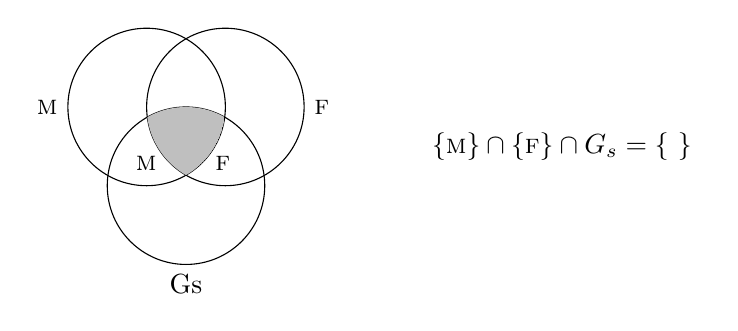
\begin{tikzpicture}[
		baseline=(current bounding box.north),
			set/.style = {
				circle,
				draw,
				minimum size = 2cm
			}
		]
		\node[set, label={180:\textsc{m}}]    (M)  at (0.0,+0.5) {};
		\node[set, label={  0:\textsc{f}}]    (F)  at (1.0,+0.5) {};
		\node[set, label={270:G\tsub{s}}] (MF) at (0.5,-0.5) {};
		\begin{scope}
			\clip (0.0,+0.5) circle(1cm);
			\clip (1.0,+0.5) circle(1cm);
			\clip (0.5,-0.5) circle(1cm);
			\fill[lightgray](0.0,+0.5) circle(1cm);
		\end{scope}
		\node at (barycentric cs:M=1,MF=1) [below left]  {\textsc{m}};
		\node at (barycentric cs:F=1,MF=1) [below right] {\textsc{f}};
		\node at (barycentric cs:M=1,F=1,MF=1) {};
		\node[anchor=west,align=left] at (3.5,0) {
			$\{\textsc{m}\} \cap \{\textsc{f}\} \cap G_s = \{\ \}$
		};
	\end{tikzpicture}
	\caption{Unbelebtes Maskulinum und Femininum kombiniert}
	\label{fig:iclgr2_1}
	\end{figure}

	\ex \label{ex:iclgr2_2}
		\gll einen Hof / vnd ein Lehen - da pei / vnd ſind paidev æigen \\
			einen Hof[\textsc{acc.sg.\MascI}] {} und ein
				Lehen[\textsc{acc.sg.\NeutI}] {} da bei {} \textsc{rel}
				sein[\textsc{3pl\subM.ind.prs}] beide-\textsc{nom.pl.\NeutI.st}
				Eigentum \\
			\trans `einen Hof und ein Lehen in der Nähe, die beide Eigentum
				sind'
				\parencites(Nr.~1923, Steyr, 1294)[194,36--37]{cao3}

	\begin{figure}
	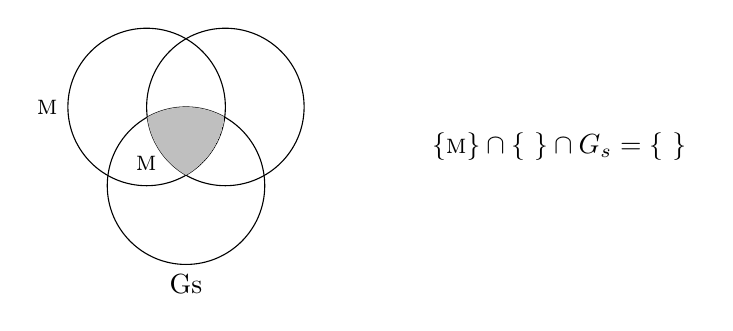
\begin{tikzpicture}[
			baseline=(current bounding box.north),
			set/.style = {
				circle,
				draw,
				minimum size = 2cm
			}
		]
		\node[set, label={180:\textsc{m}}]    (M)  at (0.0,+0.5) {};
		\node[set, label={  0:}]      (N)  at (1.0,+0.5) {};
		\node[set, label={270:G\tsub{s}}] (MF) at (0.5,-0.5) {};
		\begin{scope}
			\clip (0.0,+0.5) circle(1cm);
			\clip (1.0,+0.5) circle(1cm);
			\clip (0.5,-0.5) circle(1cm);
			\fill[lightgray](0.0,+0.5) circle(1cm);
		\end{scope}
		\node at (barycentric cs:M=1,MF=1) [below left] {\textsc{m}};
		\node at (barycentric cs:M=1,N=1,MF=1) {};
		\node[anchor=west,align=left] at (3.5,0) {
			$\{\textsc{m}\} \cap \{\ \} \cap G_s = \{\ \}$
		};
	\end{tikzpicture}
	\caption{Unbelebtes Maskulinum und Neutrum kombiniert}
	\label{fig:iclgr2_2}
	\end{figure}

	\ex \label{ex:iclgr2_3}
		\gll daz ich auz minem hauz vnd auz miner hofſtat div bediv min recht
				eigen ſint \textelp{} \\
			dass ich aus meinem Haus[\textsc{dat.sg.\NeutI}] und aus meiner
				Grundstück[\textsc{dat.sg.\FemI}] \textsc{rel.nom.pl.\NeutI}
				beide-\textsc{nom.pl.\NeutI.st} mein rehtmäßig Eigentum sind {}
				\\
			\trans `dass ich aus meinem Haus und aus meinem Grundstück, die
				beide mein rechtmäßiges Eigentum sind \textelp{}'
				\parencites(Nr.~1282, Ulm und Kl.~Raitenhaslach, Kr.~Altötting, 1282)[526,37--38]{cao2}

		\begin{figure}
		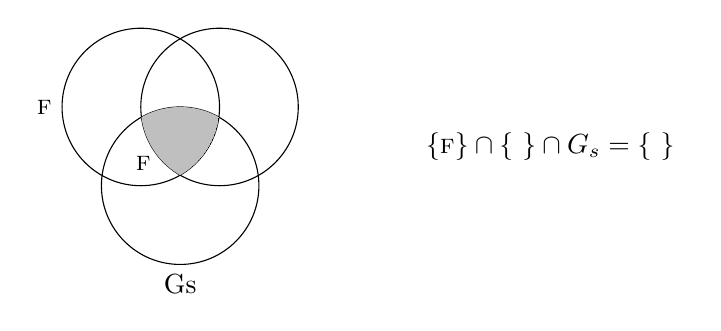
\begin{tikzpicture}[
				baseline=(current bounding box.north),
				set/.style = {
					circle,
					draw,
					minimum size = 2cm
				}
			]
			\node[set, label={180:\textsc{f}}]    (F)  at (0.0,+0.5) {};
			\node[set, label={  0:}]      (N)  at (1.0,+0.5) {};
			\node[set, label={270:G\tsub{s}}] (MF) at (0.5,-0.5) {};
			\begin{scope}
				\clip (0.0,+0.5) circle(1cm);
				\clip (1.0,+0.5) circle(1cm);
				\clip (0.5,-0.5) circle(1cm);
				\fill[lightgray](0.0,+0.5) circle(1cm);
			\end{scope}
			\node at (barycentric cs:F=1,MF=1) [below left] {\textsc{f}};
			\node at (barycentric cs:F=1,N=1,MF=1) {};
			\node[anchor=west,align=left] at (3.5,0) {
				$\{\textsc{f}\} \cap \{\ \} \cap G_s = \{\ \}$
			};
		\end{tikzpicture}
		\caption{Unbelebtes Femininum und Neutrum kombiniert}
		\label{fig:iclgr2_3}
		\end{figure}
	\end{xlist}
\end{exe}

\is{Inanimata|)}
\is{Controller|)}

\subsection{Neutrum bei maskulinem und femininem Bezug}
\label{subsec:m+m_anim_beidiu}
\is{Ausnahme|(}

Neben regelmäßigen Fällen, in denen die Kombination zweier Maskulina die Form
\norm{bėide} ergibt, zeigten sich sowohl mit Bezug auf belebte\is{Animata} als
auch auf unbelebte\is{Inanimata} maskuline (Erst-)\isi{Controller} mehrere
Vorkommen von neutralem \norm{bėidiu}. Diese verteilen sich auf alle
untersuchten Kontexte, wie beispielhaft in
(\ref{ex:m+m_beidiu_1}--\ref{ex:m+m_beidiu_5}) gezeigt, mit
Ausnahme\is{Ausnahme} der Abhängigkeit von pronominalen
Controllern\is{Controller} mit belebter Referenz. Der Beleg in
\REF{ex:m+m_beidiu_1} enthält ein \norm{bėidiu}-\isi{Target}, das sich
unmittelbar auf das Plural-Maskulinum \lit{rihtær} `Richter' bezieht, das
seinerseits männlich denotiert\is{Denotation} ist.

\begin{exe}
\ex \label{ex:m+m_beidiu_1}
	\gll Die rihtær ſprachen beideu {dar zuͦ} \\
		die Richter[\textsc{nom.pl.\MascM}] sprachen
		beide-\textsc{nom.pl.\NeutM.st} dazu \\
	\trans `Die Richter äußerten sich beide dazu'
		(%
			B1:~28ra,8; vgl.~abweichend
			\KC:~V.~10090;
			\cite[267]{schroeder1895}% 1140 mit Parallelstelle in H
		)
\end{exe}

Bei \REF{ex:m+m_beidiu_3} bezieht sich \lit{bedu} entweder direkt auf die
beiden Herren \lit{Ruͦd}\textins{\norm{iger}/\norm{olf}?} und \lit{vͦlrich}
oder auf \lit{Jungherren} `Junker'. In jedem Fall ist die Kongruenzform von
\norm{bėide} anomal.

\begin{exe}
\ex \label{ex:m+m_beidiu_3}
	\gll Diſ dingeſ gezuga ſint · Ruͦd · von der palma min Oͤhen · vͦlrich
			von Grvͤnenberch min Oͤhen bedu Jungherren \textelp{} \\
		Dies Verhandlung-\textsc{gen.sg.\NeutI} Zeugen sind {}
			\lit{Ruͦd}[\textsc{nom.sg.\MascM}] {} von der Palme mein Oheim
			{} Ulrich[\textsc{nom.sg.\MascM}] von Grünenberg mein Oheim
			beide-\textsc{nom.pl.\NeutM.st}
			Jungherren[\textsc{nom.pl.\MascM}] {} \\
	\trans `Zeugen dieser Verhandlung sind: \lit{Ruͦd} von der Palme,
		mein Onkel, Ulrich von Grünenberg, mein Onkel -- beide Junker --
		\textelp{}'
		\parencites(Nr.~2915, Kl.~St.~Urban, Kt.~Luzern, 1298)[213,33--35]{cao4}
\end{exe}

% \begin{exe}
% \ex \label{ex:m+m_beidiu_4}
% 	\gll vnſerne zehenden zeandeluingen vnde ainen Garten indem ſelben
% 			dorfe \textelp{} div wier baidiv fvr reht aigen her
% 			haigen~\textins{sic} braht \\
% 		unseren Zehnt-\textsc{acc.sg.\MascI} zu=Andelfingen und einen
% 			Garten-\textsc{acc.sg.\MascI} in.dem selben Dorf {}
% 			\textsc{rel.acc.pl.\NeutI} wir beide-\textsc{acc.pl.\NeutI.st}
% 			für rehtmäßig Eigentum her haben gebracht \\
% 	\trans `unseren Zehnten in Andelfingen und einen Garten in
% 		demselben Dorf \textelp{}, die wir beide zum rechtmäßigen Eigentum
% 		\textins{dar}gebracht haben'
% 		\parencites(Nrn.~1201~AB, Kl.~Heiligkreuztal, Kr.~Biberach, 1290)[472,10--14]{cao2}
% \end{exe}

Zuletzt bezieht sich die neutrale Form \lit{baidiv} in \REF{ex:m+m_beidiu_5}
dem Kontext nach am ehesten auf \lit{zehenden} `Zehnten' und \lit{Garten}
`Garten'. Da es sich bei den Ausstellern der Urkunde um die drei Brüder
\lit{wezel vn̄ hainrich wezel vnde Cvͦnrat de\textins{n} Bodemer}
\autocites(Nrn.~1201~AB)[472,6--7]{cao2} handelt, wird sich \lit{baidiv} nicht
auf \lit{wier} beziehen. Vielmehr wurde die Stelle so interpretiert, dass der
Zehnt und der Garten gemeinsam im Rahmen der Verkaufsverhandlung als
rechtmäßiges Eigentum dargebracht werden.

\begin{exe}
\ex \label{ex:m+m_beidiu_5}
	\gll vnſerne zehenden \textelp{} vnde ainen Garten \textelp{} div wier
			baidiv fvr reht aigen her haigen braht \\
		unseren Zehnt-\textsc{acc.sg.\MascI} {} und einen
		Garten-\textsc{acc.sg.\MascI} {} \textsc{rel.acc.pl.\NeutI} wir
		beide-\textsc{acc.pl.\NeutI.st} für rehtmäßig Eigentum her haben
		gebracht \\
	\trans `unseren Zehnten \textelp{} und einen Garten \textelp{}, die wir
		beide zum rechtmäßigen Eigentum \textins{dar}gebracht haben'
		\parencites(Nrn.~1201~AB, Kl.~Heiligkreuztal, Kr.~Biberach, 1290)[472,10--14]{cao2}
\end{exe}

Das Modell von \citet{wechsler2009} und \citet{wechslerzlatic2003} vermag diese
Ausnahmen\is{Ausnahme} nicht zu erklären. \tabref{tab:m+m_beidiu} zeigt die
Verteilung\is{Distribution!statistische} der Formen mit Bezug auf
maskulin-männliche und maskulin-unbelebte\is{Inanimata} \isi{Controller} auf
die unterschiedlichen belegten syntaktischen Kontexte. Hervorzuheben ist, dass
insgesamt lediglich neun Belege in der gesamten \isi{Stichprobe} betroffen
sind~-- sechs im ausgewertete Material des \CAO{} und weitere drei in der
Stichprobe zur \KC{}. Es handelt sich hier also eher um eine Randerscheinung.
\citet[581]{wechsler2009} und \citet[190]{wechslerzlatic2003} merken
hinsichtlich ähnlicher Fälle im \ili{BKMS} an, dass
\citet{corbett1983,corbett1991} basierend auf Textbeispielen viele
Ausnahmen\is{Ausnahme} zu seiner Resolutionsregel vermelde, insofern das
Maskulin-Plural-\isi{Default} übermäßig auf solche Kontexte\is{Pragmatik}
angewandt wird, die allein aus femininen Konjunkten bestehen.

\begin{table}
\setlength{\tabcolsep}{5pt}
\caption{Form in Bezug auf männliche bzw.\ maskuline \isi{Controller}}
\begin{tabular}{
	c c c
	r r
	c
	r r
	r
}
\lsptoprule

\mr{2}{*}[-.5ex]{\isi{Controller}}
	& \mr{2}{*}[-.5ex]{Merkmal(e)}
	& \mr{2}{*}[-.5ex]{Float\is{Floating Quantifier}}
	& \mc{2}{c}{\CAO{}}
	& %
	& \mc{2}{c}{\KC{}}
	& \mr{2}{*}[-.5ex]{Summe}
	\\

\cmidrule{4-5}
\cmidrule{7-8}

%
	& %
	& %
	& \norm{bėid(e)}
	& \norm{bėidiu}
	& %
	& \norm{bėid(e)}
	& \norm{bėidiu}
	& %
	\\

\midrule

N\tsub{i}
	& \MascM
	& $-$
	&  25 % CAO beide
	& % CAO beidiu
	& %
	&   3 % KC beide
	& % KC beidiu
	&  28 % Summe
	\\

%
	& %
	& $+$
	& % CAO beide
	& % CAO beidiu
	& %
	&   2 % KC beide
	&   2 % KC beidiu
	&   4 % Summe
	\\

\cmidrule{2-9}

%
	& \MascI
	& $-$
	&   8 % CAO beide
	& % CAO beidiu
	& %
	& % KC beide
	& % KC beidiu
	&   8 % Summe
	\\

\midrule

N\tsub{i}~+~N\tsub{j}
	& $\MascM+\MascM$
	& $-$
	& % CAO beide
	&   1 % CAO beidiu
	& %
	& % KC beide
	& % KC beidiu
	&   1 % Summe
	\\

%
	& %
	& $+$
	&   1 % CAO beide
	& % CAO beidiu
	& %
	&   2 % KC beide
	&   1 % KC beidiu
	&   4 % Summe
	\\

\cmidrule{2-9}

%
	& $\MascI+\MascI$
	& $+$
	& % CAO beide
	&   1 % CAO beidiu
	& %
	& % KC beide
	& % KC beidiu
	&   1 % Summe
	\\

\midrule

PRO\tsub{i}
	& \MascM
	& $-$
	&   3 % CAO beide
	& % CAO beidiu
	& %
	& % KC beide
	& % KC beidiu
	&   3 % Summe
	\\

%
	& %
	& $+$
	& % CAO beide
	& % CAO beidiu
	& %
	&   7 % KC beide
	& % KC beidiu
	&   7 % Summe
	\\

\midrule

PRO\tsub{i+j}
	& $\MascM+\MascM$
	& $-$
	&  15 % CAO beide
	& % CAO beidiu
	& %
	&   1 % KC beide
	& % KC beidiu
	&  16 % Summe
	\\

%
	& %
	& $+$
	&  10 % CAO beide
	& % CAO beidiu
	& %
	&  12 % KC beide
	& % KC beidiu
	&  22 % Summe
	\\

\cmidrule{2-9}

%
	& $\MascI+\MascI$
	& $-$
	& % CAO beide
	&   1 % CAO beidiu
	& %
	& % KC beide
	& % KC beidiu
	&   1 % Summe
	\\

%
	& %
	& $+$
	&   2 % CAO beide
	&   3 % CAO beidiu
	& %
	& % KC beide
	& % KC beidiu
	&   5 % Summe
	\\

\midrule

\mc{3}{l}{Summe}
	&  64 % CAO beide
	&   6 % CAO beidiu
	& %
	&  27 % KC beide
	&   3 % KC beidiu
	& 100 % Summe
	\\

\lspbottomrule	
\end{tabular}
\label{tab:m+m_beidiu}
\end{table}

Auf die Situation im Mittelhochdeutschen\il{Mittelhochdeutsch} übertragen ist
anzunehmen, dass das Neutrum als Resolutionsgenus\is{Gender Resolution} auf die
anderen beiden Geschlechter übergreift. In den hier ausgewerteten Quellen lässt
sich dies für das Femininum aufgrund fehlender Belege nicht nachvollziehen,
wohl aber für das Maskulinum. Mit Verweis auf \citet[302]{corbett1991}
schreiben \citet[581]{wechsler2009} und \citet[190]{wechslerzlatic2003} weiter,
dass dieser bemerke, keine Beispiele für maskuline Kongruenz mit femininen
Nomina, die sich auf Personen beziehen, gefunden zu haben. Sie schließen
daraus, dass (zumindest im \ili{BKMS}) mit Kongruenz entgegen dem Sexus
belebter\is{Animata} Referenten nicht zu rechnen ist, während die schwächere,
abgeleitete Resolutionsregel für unbelebte\is{Inanimata} Referenten
gelegentlich verletzt wird.

Aus \tabref{tab:m+m_beidiu} ergibt sich, dass \norm{bėidiu} mit männlichem
Bezug im \CAO{} nur in Kontexten mit kombinierter Referenz auftritt, sowohl bei
direktem als auch indirektem Bezug auf die \isi{Controller} und sowohl in
\isi{Kontaktstellung} als auch in \isi{Distanzstellung}. Zwei Belegen mit
belebt-männlicher Referenz stehen vier mit unbelebt-maskuliner\is{Inanimata}
gegenüber. In der \KC{} dagegen tritt \norm{bėidiu} nur beim direkten Bezug
auf, dafür aber sowohl in Kontexten mit kombinierter als auch einfacher
Referenz, und nur in \isi{Distanzstellung}. \isi{Inanimata} sind in der
\isi{Stichprobe} zur \KC{} nicht vertreten. Abgesehen davon, dass für die \KC{}
nur drei verwendbare Belege vorliegen gegenüber den sechs Belegen beim \CAO{},
verhalten sich beide Datenserien konträr zueinander\is{Validierung}.

Dadurch, dass neutrales \norm{bėidiu} mit maskuliner Referenz hauptsächlich mit
unbelebten\is{Inanimata} Controllern\is{Controller} einhergeht, gilt zumindest
für das \CAO{} eingeschränkt die oben zitierte Schlussfolgerung, dass sich das
Übergreifen des Resolutionsgenus\is{Gender Resolution} in solchen Kontexten
bemerkbar mache, in denen die formale Ausgleichsregel bei \isi{Inanimata}
eintritt, wie in \REF{ex:gendasshier} beschrieben. Die zweite Hälfte der These,
dass dies nur bei unbelebten\is{Inanimata} Targets\is{Target} der Fall sei,
trifft auf die Beleglage im \CAO{} nicht ganz zu, und gar nicht auf die \KC{}.
Aus dem synchronen System des Mittelhochdeutschen\il{Mittelhochdeutsch} um 1300
heraus ist jedenfalls formal nicht nachvollziehbar\is{Validierung}, warum zwei
Maskulina in manchen Fällen kombiniert als Neutrum aufgenommen werden.

Während im untersuchten Material keine Kombination von zwei
unbelebten\is{Inanimata} Feminina vorkommt (bezogen auf die Kombination von
belebten\is{Animata} Feminina steht immer \norm{bėide}), gibt
\citet[384]{paul2007} zur Illustration den in \REF{ex:walther92_25-28_C_2}
zitierten Beleg an. Dort steht in Bezug auf die Abstrakta \lit{liͤbe} `Liebe'
und \lit{ſchoͤne} `Schönheit' das Demonstrativum\is{Demonstrativpronomen}
\lit{diſiu̍} `diese', das zumindest der Form nach als Neutrum erscheint
\autocite[485]{ksw2}. Das folgende \lit{beide} hat dagegen eine Form, die der
Annahme von femininer Kongruenz zumindest nicht entgegen steht.

\begin{exe}
\ex\label{ex:walther92_25-28_C_2}
	\gll du̍ liͤbe ſtet der ſchoͤne bi~· \\
			die Liebe[\textsc{nom.sg.\FemI}] steht der
			Schönheit[\textsc{dat.sg.\FemI}] bei \\
\sn \gll bas danne geſteine dē golde tvͦt~· \\
		besser als Edelstein dem Gold tut \\
\sn \gll nv iehet wc danne beſſer ſi~· \\
		nun sprecht was daher besser sei \\
\sn \gll hant diſu̍ beide rehten mvͦt~· \\
		haben dies-\textsc{nom.pl.\NeutI.st} beide-\textsc{nom.pl.m+f\subI.st}
			gehörigen Gesinnung \\
	\trans `Die Liebe passt zur Schönheit besser als die Edelsteine zum
		Gold: Nun sprecht, was daher besser sei, wenn diese beide gehöriger
		Gesinnung sind.'
		(%
			\iai{Walther von der Vogelweide}: 92,25--28 nach
			Heidelberg, Universitätsbibl., Cod.~Pal.~germ.~848: 128rb,1--4;
			% [\cite[4957]{hsc}],
			vgl.~\cite[356--358]{bein2013}%
		)
	\\
\end{exe}

\cite[485]{ksw2} merken an, dass Formen vom Typ \norm{disiu} in
alemannischen\il{Alemannisch} Quellen \blockquote{\textins{v}ereinzelt auch im
Nom.Pl.Fem.} auftreten -- es wird angenommen, dass der Kodex Manesse im
Raum\is{Dialektgeografie} Zürich um 1300 entstand \autocite[4957]{hsc}.
\Citet[27]{deboor1976b} attestiert alemannischen\il{Alemannisch}
Urkundenschreibern \blockquote{Anzeichen von Unsicherheit in der richtigen
Verwendung von \norm{disiu}}. Er vermutet, dass sie
\blockcquote[28]{deboor1976b}{\norm{disiu} \textins{schrieben}, wie sie es
gelernt hatten, wo in der mündlichen\is{Mündlichkeit} Verhandlung schon
\norm{dise} gesprochen wurde, und es passierte ihnen, daß sie \norm{disiu}
schrieben\is{Schriftlichkeit}, auch wo \norm{dise} richtig war}.

Unter einer geografischen\is{Dialektgeografie} Perspektive ist festzustellen,
dass die \CAO{}-Belege zu Neutrum mit Bezug auf Maskulina aus Augsburg,
Freiburg i.\,Br., dem Kloster Heiligkreuztal (Kr.~Biberach) und dem Kloster
St.~Urban (Kt.~Luzern) stammen. Diese Orte liegen alle im
alemannischen\il{Alemannisch} und schwäbischen\il{Schwäbisch} Gebiet. Im Fall
der \KC{} sind die Handschriften K und B1 aus dem alemannischen\il{Alemannisch}
und mittelbairischen\il{Bairisch} Sprachraum\is{Dialektgeografie} betroffen.
Damit stammen insgesamt sieben Belege für dieses Phänomen aus dem West- und
zwei aus dem Ost\-ober\-deutschen\il{Bairisch}.

Festzuhalten ist, dass sich in alemannischen\il{Alemannisch} Urkunden des
späten 13.~Jahrhunderts ein Schwanken zwischen \norm{dise} und \norm{disiu}
beobachten lässt, das auch den Beleg in \REF{ex:walther92_25-28_C_2} erklären
könnte. Es lässt sich annehmen, dass das ursprüngliche System der
Pluralkongruenz im \isi{Genus} durch die Ausweitung der maskulin-femininen
Form\is{Genusdistinktion, Abbau der} für Schreiberinnen und Schreiber aus dem
alemannischen\il{Alemannisch} Gebiet um 1300 nicht mehr klar erkennbar war.

\is{Ausnahme|)}

\subsection{Zusammenfassung}

Zur theoretischen Reflexion der ausgewerteten Belege aus dem \CAO{} und der
\KC{} wurde das in \citet{wechsler2009} und \citet{wechslerzlatic2003}
vorgestellte Modell zur Erklärung herangezogen. Dieses basiert auf der
LFG\is{Lexical-functional Grammar} und fasst \isi{Gender Resolution} als
Schnittmengenoperation auf. Die von \citet[578]{wechsler2009} und
\citet[186]{wechslerzlatic2003} für das moderne Isländische\il{Isländisch}
formulierten Regeln lassen sich auch auf den Großteil der gesammelten
mittelhochdeutschen\il{Mittelhochdeutsch} Belege anwenden.

Der Bezug von \norm{bėide} auf einzelne Substantive\is{Substantiv} im Plural --
sowohl direkt als auch indirekt -- bereitete keine Probleme. Die Belege zeigen
bis auf wenige Ausnahmen\is{Ausnahme} regelmäßig formale
Kongruenz\is{Kongruenz!formale}. Interessant, aber nicht durch die gesammelten
Belege zu erörtern, ist die Frage, ob bei direktem Bezug auf ein Hybrid Noun
wie \norm{wīp} `Frau (\NeutF)' als \isi{Controller} beim \isi{Target} in
gefloateter\is{Floating Quantifier} Position eher formale\is{Kongruenz!formale}
(\norm{-iu}) oder semantische Kongruenz\is{Kongruenz!semantische} (\norm{-e})
eintritt, das heißt, ob eher Genus\is{Genusmerkmal} oder Sexus\is{Sexusmerkmal}
das wichtigere Merkmal bei der Kongruenz darstellt.%
%
	\footnote{Belege dafür sind überraschend schwierig zu finden. Eine Suche
		sowohl im \CAO{} als auch in den als oberdeutsch klassifizierten Texten
		des \REM{} nach dem Lemma \norm{wīp} (Kodierung: \emph{wîp}) im Plural
		gefolgt von dem Lemma \norm{bėide} (Kodierung: \emph{bèide}) im
		Nom./Akk. im Abstand bis zu zehn Wortformen\is{Distanz!lineare}
		lieferte keine Ergebnisse.}

Besteht der \isi{Controller} von \norm{bėide} aus kombinierten Nominalen, das
heißt, sowohl Substantiven\is{Substantiv} als auch Pronomina der ersten oder
selten der zweiten Person, wird ein Konflikt von
Geschlechtsmerkmalen\is{Sexusmerkmal} beim direkten Bezug regelmäßig semantisch
aufgelöst. Ein männlich und ein weiblich denotierter\is{Denotation}
\isi{Controller} ergeben zusammen also eine Form vom Typ \norm{bėidiu} und
damit ein Neutrum. Etwas differenzierter ist die Lage bei den Belegen mit
indirektem Bezug zwischen \isi{Controller} und \isi{Target}. Hier steht in der
Regel ein Personal-\is{Personalpronomen} oder
Relativpronomen\is{Relativpronomen} zwischen \isi{Erstcontroller} und
\norm{bėide}-Target. Das Pronomen selbst ist damit sowohl Target als auch
\isi{Controller}, wie in dem Schema in
\figref{fig:beid2p2coordn} illustriert.

Beim indirekten Bezug auf unbelebte\is{Inanimata} \isi{Erstcontroller} kommt
sehr regelmäßig der von \citet[577]{wechsler2009} und
\citet[184]{wechslerzlatic2003} vorgeschlagene Algorithmus zur Anwendung:
Maskulinum und Femininum sind respektive als $\{\textsc{m}\}$ und
$\{\textsc{f}\}$ definiert; das Neutrum als Resolutionsgenus\is{Gender
Resolution} ist eine leere Menge $\{\ \}$; Maskulinum und Femininum als formale
Korrelate der semantischen Genera\is{Genus} (männlich und weiblich) bilden
zusammen die Menge G\tsub{s}. Die Kongruenzform ergibt sich dann durch die
dreifache Schnittmenge der Genera\is{Genus} der beiden \isi{Erstcontroller} und
G\tsub{s}. Ist die Schnittmenge leer, tritt das Neutrum auf. Aufgrund des
Fehlens von Belegen zu kombinierten unbelebten\is{Inanimata} Feminina kann
keine Aussage darüber gemacht werden, ob die Regel auch in diesem Fall
zutrifft. Regelmäßig zu erwarten wäre dem Modell nach feminine Kongruenz.

Die Belege für Targets\is{Target} mit indirektem Bezug auf belebte\is{Animata}
\isi{Erstcontroller} weisen insgesamt die größte Variation zwischen
\norm{bėide} und \norm{bėidiu} auf. In rund 65\,\% aller Fälle hängt das Target
direkt von einem \isi{Personalpronomen} ab, in aller Regel \norm{si} oder
\norm{wir}. Das Personalpronomen ist in allen untersuchten Kontexten
genusneutral\is{Genusindifferenz}, gibt also selbst keine formale Bedingung für
Kongruenz vor, während darauf bezogenes \norm{bėide} kongruieren muss. Es wurde
argumentiert, dass bei gemischtgeschlechtlichen
Erstcontrollern\is{Erstcontroller} zwei Lösungsstrategien in Frage kommen.

Im häufigsten Fall wird semantische Kongruenz\is{Kongruenz!semantische} mit der
zu erwartenden Resolutionsregel angewandt: Gemischter männlicher und weiblicher
Bezug wird durch eine neutrale Form mit \mbox{\norm{-iu}} semantisch aufgelöst.
Im weniger häufigen Fall wird das \isi{Sexusmerkmal} dem Anschein nach formal
aufgelöst, insofern \norm{-e} auf formaler Ebene Maskulinum und Femininum
umfasst. Die Variation lässt sich so auf divergierende grammatikalische
Präferenzen von Schreiberinnen und Schreibern zurück\-führen. Zu beobachten war
weiterhin, dass sich diese Art von Variation hauptsächlich auf Kontexte
beschränkt, in denen \norm{bėide} -- zumindest der naheliegendsten
Interpretation nach -- zusammen mit seinem \isi{Controller} eine Phrase
bildet\is{Nominalgruppe}, also Kontexte, in denen formale
Kongruenz\is{Kongruenz!formale} vorherrscht.

In Kontexten, in denen das \isi{Target} als \isi{Floating Quantifier}
klassifiziert wurde, ist dagegen regelmäßig semantische
Kongruenz\is{Kongruenz!semantische} zu finden, insofern sehr regelmäßig
\isi{Gender Resolution} auftritt. Beim Bezug auf \norm{die/diu} als
Relativpronomen\is{Relativpronomen} haben sich dort, wo das Pronomen seiner
Form gemäß ein formales Genusmerkmal\is{Genusmerkmal} definiert, keine Fälle
bemerkbar gemacht, in denen die Form von \norm{bėide} im Widerspruch dazu
stehen würde.

Bezogen auf die Untersuchung der Kongruenz von \norm{bėide} in Abhängigkeit von
Pro\-nomen der 3.~Person erscheint es angebracht,\is{Desiderat} ältere Quellen
als die Urkunden des \CAO{} und die \KC{}-Handschriften B1, C1, K und VB (alle
13. oder 14.~Jahrhundert, vgl.~\figref{fig:zeitstrahl}) auf das Auftreten von
unerwarteten Kombinationen wie \norm{sie bėidiu} oder \norm{siu bėide} hin zu
untersuchen. In den genannten \KC{}-Handschriften sind nur \norm{si bėide/-iu}
sowie \norm{di/die bėide} belegt (vgl.~\sectref{subsubsec:monoflexionkc}). Die
semantische Kongruenz\is{Kongruenz!semantische} bei Distanz\-stellung
betreffend wäre eine Untersuchung althochdeutscher\il{Althochdeutsch} Quellen
interessant\is{Desiderat}, da dort prädikative
Adjektive\is{Adjektiv!prädikativ} zum Teil noch flektiert
werden.\is{Kongruenz!prädikative} \citet[310--311]{fleischer2007} zufolge
zeigen insgesamt rund ein Fünftel der Belege in seiner \isi{Stichprobe}
Flexion, wobei Kontexte mit semantischer Kongruenz und solche, bei denen die
Kongruenzform des Adjektivs nicht mit seinem Subjekt übereinstimmt,
ausgeschlossen wurden \autocite[304]{fleischer2007}.

Neben der Mehrheit von Belegen, bei denen in Zusammenhang mit zwei Männern oder
dem Bezug auf ein \isi{Substantiv}, das eine Gruppe von Männern bezeichnet,
regulär die maskuline Form \norm{bėid(e)} auftritt, liegen im exzerpierten
Material insgesamt neun Belege vor, in denen unregelmäßig\is{Ausnahme} die
neutrale Form \norm{bėidiu} in demselben Kontext auftritt. Eine
morphosyntaktische Begründung hierfür konnte nicht gefunden werden. Der
Erklärungsansatz für \isi{Gender Resolution} von \citet{wechslerzlatic2003} und
\citet{wechsler2009} sieht Belege dieser Art nicht vor.

Das Phänomen des Übergreifens der Resolutionsform auf an sich unproblematische
Kontexte wird aber auch von \citet[302]{corbett1991} bei seiner Untersuchung
von Belegen aus dem \ili{BKMS} dokumentiert. Dort greift das Maskulin als
Resolutionsform in bestimmten Fällen auch auf Kon\-texte mit kombinierten
femininen \isi{Inanimata} über. Auch in den \CAO{}-Belegen sind hauptsächlich
\isi{Inanimata} betroffen. Vermutlich wird analog zum \ili{BKMS} das Neutrum
als Resolutionsgenus\is{Gender Resolution} auch von manchen
mittelhochdeutschen\il{Mittelhochdeutsch} Schreiberinnen und Schreibern als
Form der kombinierten Referenz übergeneralisiert\is{Generalisierung}, besonders
bei unbelebtem\is{Inanimata} Bezug, doch möglicherweise nicht ausschließlich,
wie zumindest zwei \KC-Belege zeigen.

%%%%%%%%%%%%%%%%%%%%%%%%%%%%%%%%%%%%%%%%%%%%%%%%%%%%%%%%%%%%%%%%%%%%%%%%%%%%%%%

\section{\norm{Bėide} als Konjunktion}
\label{sec:beideconj}
\is{Konjunktion|(}
\is{Koordination|(}

Für das Mittelhochdeutsche\il{Mittelhochdeutsch} sprechen sich
\citet[626--627]{ksw2} klar dafür aus, dass \norm{bėidiu} als Bestandteil der
korrelativen Konjunktion \norm{bėidiu \dots\ unde} `sowohl \dots\ als auch' in
dieser Form erstarrt ist, also \norm{bėidiu} entgegen der Annahme von
\citet{askedal1974} nicht entsprechend den Genusmerkmalen\is{Genusmerkmal}
seiner Konjunkte flektiert (\sectref{sec:ovwbeideconj}). Nimmt man dennoch an,
dass im Zusammenspiel mit nominalen Konjunkten innerhalb der Konstruktion
Closest Conjunct Agreement\is{Closest Conjunct Agreement} auftritt, wäre zu
erwarten, dass \norm{bėide} als Teil der \isi{Nominalgruppe} wie ein
\isi{Adjektiv} oder \isi{Determinierer} entsprechend den formalen
Merkmalen\is{Merkmale!grammatische} Kasus, \isi{Genus} und \isi{Numerus} des
ersten Konjunkts flektiert (\sectref{sec:gendres}). In diesem Fall müsste
größere Formenvielfalt als bloß der Wechsel zwischen \norm{bėide} und
\norm{bėidiu} zu beobachten sein.

Im vorliegenden Belegmaterial hat die Konjunktion allerdings unabhängig von den
grammatischen Merkmalen\is{Merkmale!grammatische} der Konjunkte in ihrem
\isi{Skopus} entweder die Form \norm{bėide} oder \norm{bėidiu}. In
\REF{ex:caoconjbeide} steht daher eine Form vom Typ \norm{bėidiu}, obwohl die
Konjunkte im Dativ Singular \REF{ex:caoconjbeide_1} beziehungsweise im Genitiv
Singular \REF{ex:caoconjbeide_2} stehen. Wenn Closest Conjunct
Agreement\is{Closest Conjunct Agreement} zuträfe, wäre an diesen Stellen mit
Formen wie *\norm{bėider} (Dat.~Sg.~F.~st.) und *\norm{bėides}
(Gen.~Sg.~M.~st.) zu rechnen. Im Fall von Pluralkongruenz mit beiden Konjunkten
entsprechend einem kataphorisch-pronominalen\is{Katapher} Gebrauch von
\norm{bėide} müssten *\norm{bėiden} (Dat.\ Pl.\ st.) und *\norm{bėider} (Gen.\
Pl.\ st.) vorliegen.

\begin{exe}
\ex \label{ex:caoconjbeide}
	\begin{xlist}
	\ex \label{ex:caoconjbeide_1}
		\gll beidiu Einwige vnd auch dem kloͤſter \\
				beide Einwig-\textsc{dat.sg.\FemF} und auch
				\textsc{def.dat.sg.\NeutM} Kloster \\
		\trans `sowohl Einwig als auch dem Kloster'
			\parencites(Nr.~2925, Landshut, 1298)[219,34]{cao4}

	\ex \label{ex:caoconjbeide_2}
		\gll bédvͥ herne heſſin / vnde herne Rvͦdolfeſ \\
			beide Herr-\textsc{gen.pl.\MascM} Hesse-\textsc{gen.sg.\MascM} {}
				und Herr-\textsc{gen.pl.\MascM} Rudolf-\textsc{gen.pl.\MascM}
				\\
		\trans `sowohl Herrn Hesses als auch Herrn Rudolfs'
			\parencites(Nr.~1318, Freiburg i.\,Br., 1290)[561,11--12]{cao2}
	\end{xlist}
\end{exe}

Bei der Konjunktion \norm{bėide} handelt es sich um einen typischen Fall von
\isi{Grammatikalisierung} \autocite[vgl.][134--188]{lehmann2015}. Ermöglicht
wird diese durch grammatische Kipppunkte wie die in \sectref{sec:ovwbeideconj}
zu dem in \REF{ex:beidejohahd_2_copy} wiederholten Beispiel bemerkte Unschärfe
in der Interpretation\is{Ambiguität}. Mit zunehmender Verwendung einer Form in
einem bestimmten Kontext geht durch Konventionalisierung\is{Konvention} eine
Desemantisierung einher, ebenso verliert das lexikalische Zeichen mit der
Funktionalisierung durch das grammatische System an \q{Substanz}. Dies kann
sowohl auf phonologischer als auch auf morphosyntaktischer Ebene geschehen.

\begin{exe}
\ex \label{ex:beidejohahd_2_copy}
	\langinfo%
		{Althochdeutsch}%
		{}%
		{\cite[35]{tax1979}}\\
	\gll Trúhten besuôchet pêide · guôten ioh úbelen \\
			Herr befragt beide-\textsc{acc.pl.\MascA.st} {}
				Gut-\textsc{acc.sg.\MascA.wk} und
				Böse-\textsc{acc.sg.\MascA.wk} \\
		\trans `Der Herr befragt beide, den Guten und den Bösen.'
			(%
				\iai{Notker~III.\ von St.~Gallen}, \tit{Psalter}: 10,6%
				% = Vulgata Ps LXX 10,6 ~ Luther Ps 11,5
			)
\end{exe}

Von den morphosyntaktischen Parametern, die \citet[174]{lehmann2015} auflistet,
ist im hier beschriebenen Fall besonders eine Abnahme der
paradigmatischen\is{Paradigma} Variabilität (\fw{paradigmatic variability};
\cite[146--150]{lehmann2015}) zu beobachten. Der Quantor erstarrt in einem
Kontext, in dem er attributiv flektieren\is{Kongruenz!attributive} könnte
\REF{ex:caoconjbeide}. Dies ermöglicht eine Ausweitung des Benutzungskontexts,
hier vor allem in syntaktischer Hinsicht (\fw{dropping of selection
restrictions}; \cite[150--151]{lehmann2015}). Ein Element, das ansonsten
nominale Kategorien modifiziert und entsprechend flektiert, kann vom Zwang zur
Flexion befreit auch zusammen mit nicht-nominalen Kategorien wie
Präpositionalphrasen\is{Präpositionalphrase} (PPs) oder
Adverbialen\is{Adverbial} verwendet werden, die selbst keine mit dem Quantor
kompatiblen grammatischen Merkmale\is{Merkmale!grammatische} bieten.

Auf phonologischer Ebene könnte es sich mit \citet[134--136]{lehmann2015} bei
\norm{bėide} um phonologische Erosion (\fw{phonological attrition}) handeln,
die mit \isi{Grammatikalisierung} einhergeht, möglicherweise auch im Kontext
der \isi{Nebensilbenabschwächung} \autocite[88--92]{braune2018}. Parallel dazu
steht der Verlust der Genusopposition\is{Genusdistinktion, Abbau der} im Plural
bis zum 15.~Jahrhundert
\autocites[203]{paul2007}[191--192]{reichmannwegera1993}. Dieser macht sich bei
der starken \isi{Adjektivdeklination} in den jüngeren ausgewerteten
\KC{}-Handschriften bereits bemerkbar, in den Urkunden\is{Urkunde} jedoch noch
nicht.

In \sectref{subsec:caobeidquantsyncont} und \sectref{subsec:kcbeidquantsyncont}
wurde der Gebrauch von \norm{bėide} mit adverbialen\is{Adverbial} Konjunkten
diskutiert. Während die Präpositionalobjekte in \REF{ex:caokoordsyn_3_2} und
\figref{fig:caokoordsyn_3_2} zwar jeweils Personenmerkmale\is{Personenmerkmal}
bieten und nach dem Kasus flektieren, den die Präposition regiert, steht
\lit{baidev} nicht im Dativ. In \REF{ex:syntintvar1_2} und
\figref{fig:syntintvar1_2} enthalten die Konjunkte keinerlei
Genusmerkmale\is{Genusmerkmal}, nach denen \lit{Beideu} flektieren könnte.

\begin{exe}
\ex \label{ex:beidquantsyncont}
	\begin{xlist}
	\ex \label{ex:caokoordsyn_3_2}
		\gll baidev \textup{[\tsup{PP}} zv Dorfe \textup{]} vnd
				\textup{[\tsup{PP}} ze velde \textup{]} \\
			beide {} zu Dorf-\textsc{dat.sg} {} und {} zu Feld-\textsc{dat.sg}
				{} \\
		\trans `sowohl im Dorf als auch auf dem Feld'
			\parencites(Nr.~3319, Michelstetten, Bz.~Mistelbach, 1299)[461,28]{cao4}

		\begin{figure}
		\avm{[
			preconj	& \textit{beide} \\
			conj		& \textit{und} \\
			\{[
				pred	& \astruct{zu}{\ups{\SObj{loc}}} \\
				\SObj{loc}	& [
					pred	& `Dorf' \\
					case	& \textsc{dat} \\
					gend	& \textsc{n} \\
					anim	& $-$ \\
					num	& \textsc{sg} \\
				]
			],
			[
				pred	& \astruct{zu}{\ups{\SObj{loc}}} \\
				\SObj{loc}	& [
					pred	& `Feld' \\
					case	& \textsc{dat} \\
					gend	& \textsc{n} \\
					anim	& $-$ \\
					num	& \textsc{sg} \\
				]
			]\}
		]}
		\caption{Analyse des Satzfragments \norm{bėidiu ze dorfe unde ze velde} `sowohl im Dorf als auch auf dem Feld'}
		\label{fig:caokoordsyn_3_2}
		\end{figure}

	\ex \label{ex:syntintvar1_2}
		\gll Beideu {\ob}\tsup{AP} ſpæt {\cb} vnde
			{\ob}\tsup{AP} vruͦ {\cb} \\
			beide {} spät {} und {} früh {} \\
		\trans `sowohl spät als auch früh'
			(%
				B1:~19va,15; vgl.
				VB:~33ra,36%
			)

		\begin{figure}
		\avm{[
			preconj	& \textit{beide} \\
			conj		& \textit{und} \\
			\{[
				pred	& `spät' \\
				deg	& $pos$
			],
			[
				pred	& `früh' \\
				deg	& $pos$
			]\}
		]}
		\caption{Analyse des Satzfragments \norm{bėidiu spǟte unde vrüje} `sowohl spät als auch früh'}
		\label{fig:syntintvar1_2}
		\end{figure}
	\end{xlist}
\end{exe}

Die Annahme erscheint daher sinnvoll, dass es desemantisiert als
\isi{Fokuspartikel} dient, die betont, dass zwei gleichwertige Optionen
vorliegen \autocite[425--428]{johannessen2005}. Wie
\REF{ex:beideintiahd_3_copy} exemplarisch zeigt, ist die Verwendung von
\norm{bėide} als Konjunktion zumindest mit PPs schon in
vormittelhochdeutscher\il{Althochdeutsch} Zeit möglich.

\begin{exe}
\ex \label{ex:beideintiahd_3_copy}
	\langinfo%
		{Althochdeutsch}
		{}
		{\cite[171]{steinmeyer1916}}\\
	\gll pediu in demo lihnamen unte in demo muôte \\
		beide in \textsc{def.dat.sg.\MascI} Körper-\textsc{dat.sg.\MascI} und in
			\textsc{def.dat.sg.\MascI} Geist-\textsc{dat.sg.\MascI} \\
	\trans `sowohl im Körper als auch im Geist'
		(%
			\tit{Predigtsammlung~B}: 3,25--26%
		)
\end{exe}

Da kein morphosyntaktisches Merkmal greifbar ist, das für die
Verteilung\is{Distribution!statistische} von \norm{bėide}- und
\norm{bėidiu}-Typen der Konjunktion verantwortlich gemacht werden kann, wurde
zuvor die Frage gestellt, ob sich die Variation im Kartenbild bemerkbar macht.
\figref{fig:cao_beideconj_geo_1} und \ref{fig:cao_beideconj_geo_2} zeigen die
jeweilige geografische\is{Dialektgeografie} Verbreitung der beiden Typen
aufgrund der aus dem \CAO{} gewonnenen Belege. Während \norm{bėidiu} im ganzen
oberdeutschen\il{Oberdeutsch} Sprachraum\is{Dialektgeografie} verbreitet ist,
finden sich Belege für \norm{bėide} im Alemannischen,\il{Alemannisch}
Ostfränkischen\il{Ostfränkisch} und im Osten des Mittelbairischen\il{Bairisch}.
Überall dort kommt es zu einem Nebeneinander beider Formen. Dies deckt
sich\is{Validierung} mit den Daten von \citet[627]{ksw2}, die für die zweite
Hälfte des 13.~Jahrhunderts sowohl für das Alemannische\il{Alemannisch} als
auch für das Bairische 89\,\% \norm{bėidiu} verzeichnen, für das
Übergangsgebiet dazwischen aber 100\,\% (für das Ostfränkische\il{Ostfränkisch}
liegen für diesen Zeitabschnitt keine Daten vor).

\begin{figure}
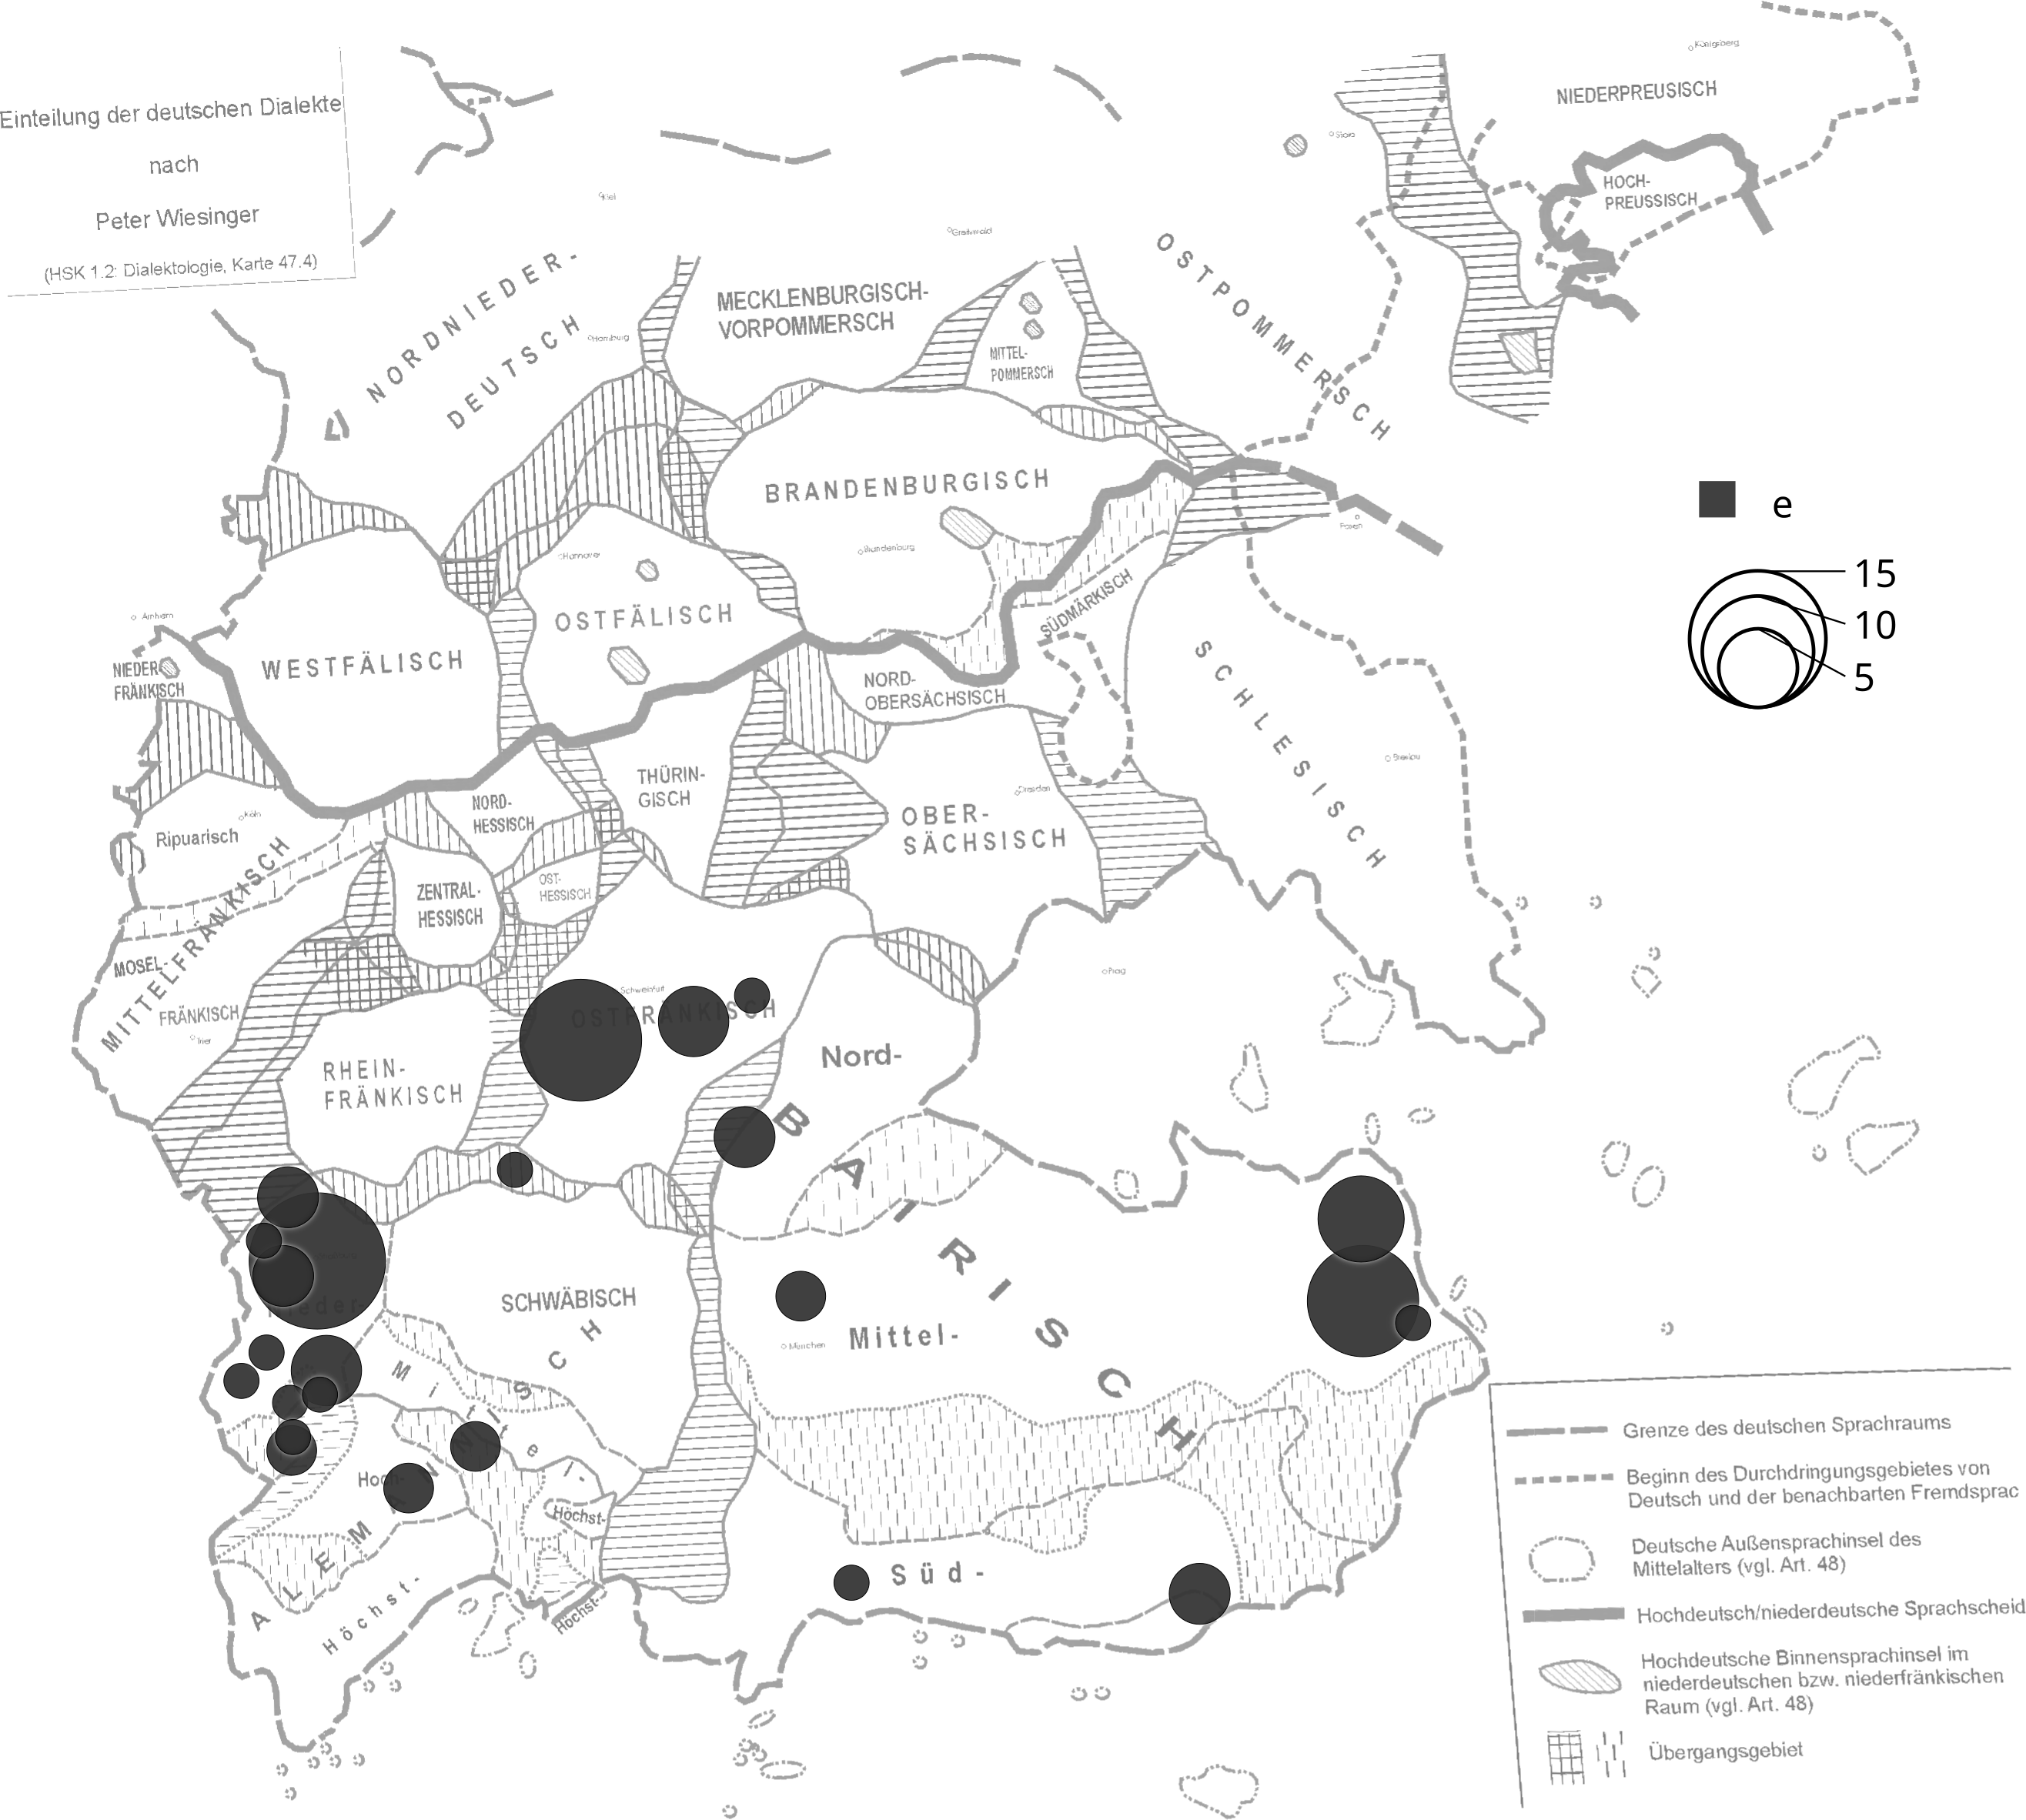
\includegraphics[
	width=\linewidth,
	keepaspectratio
]{./figures/2021-10-11_cao_beide-conj.png}
\caption{Geografische\is{Dialektgeografie}
	Distribution\is{Distribution!geografische} der Form \norm{bėide} in
	\norm{bėide \dots\ unde} `sowohl \dots\ als auch' (Hintergrundkarte:
	\cite{wiesinger1983:rede})}
\label{fig:cao_beideconj_geo_1}
\end{figure}

\begin{figure}
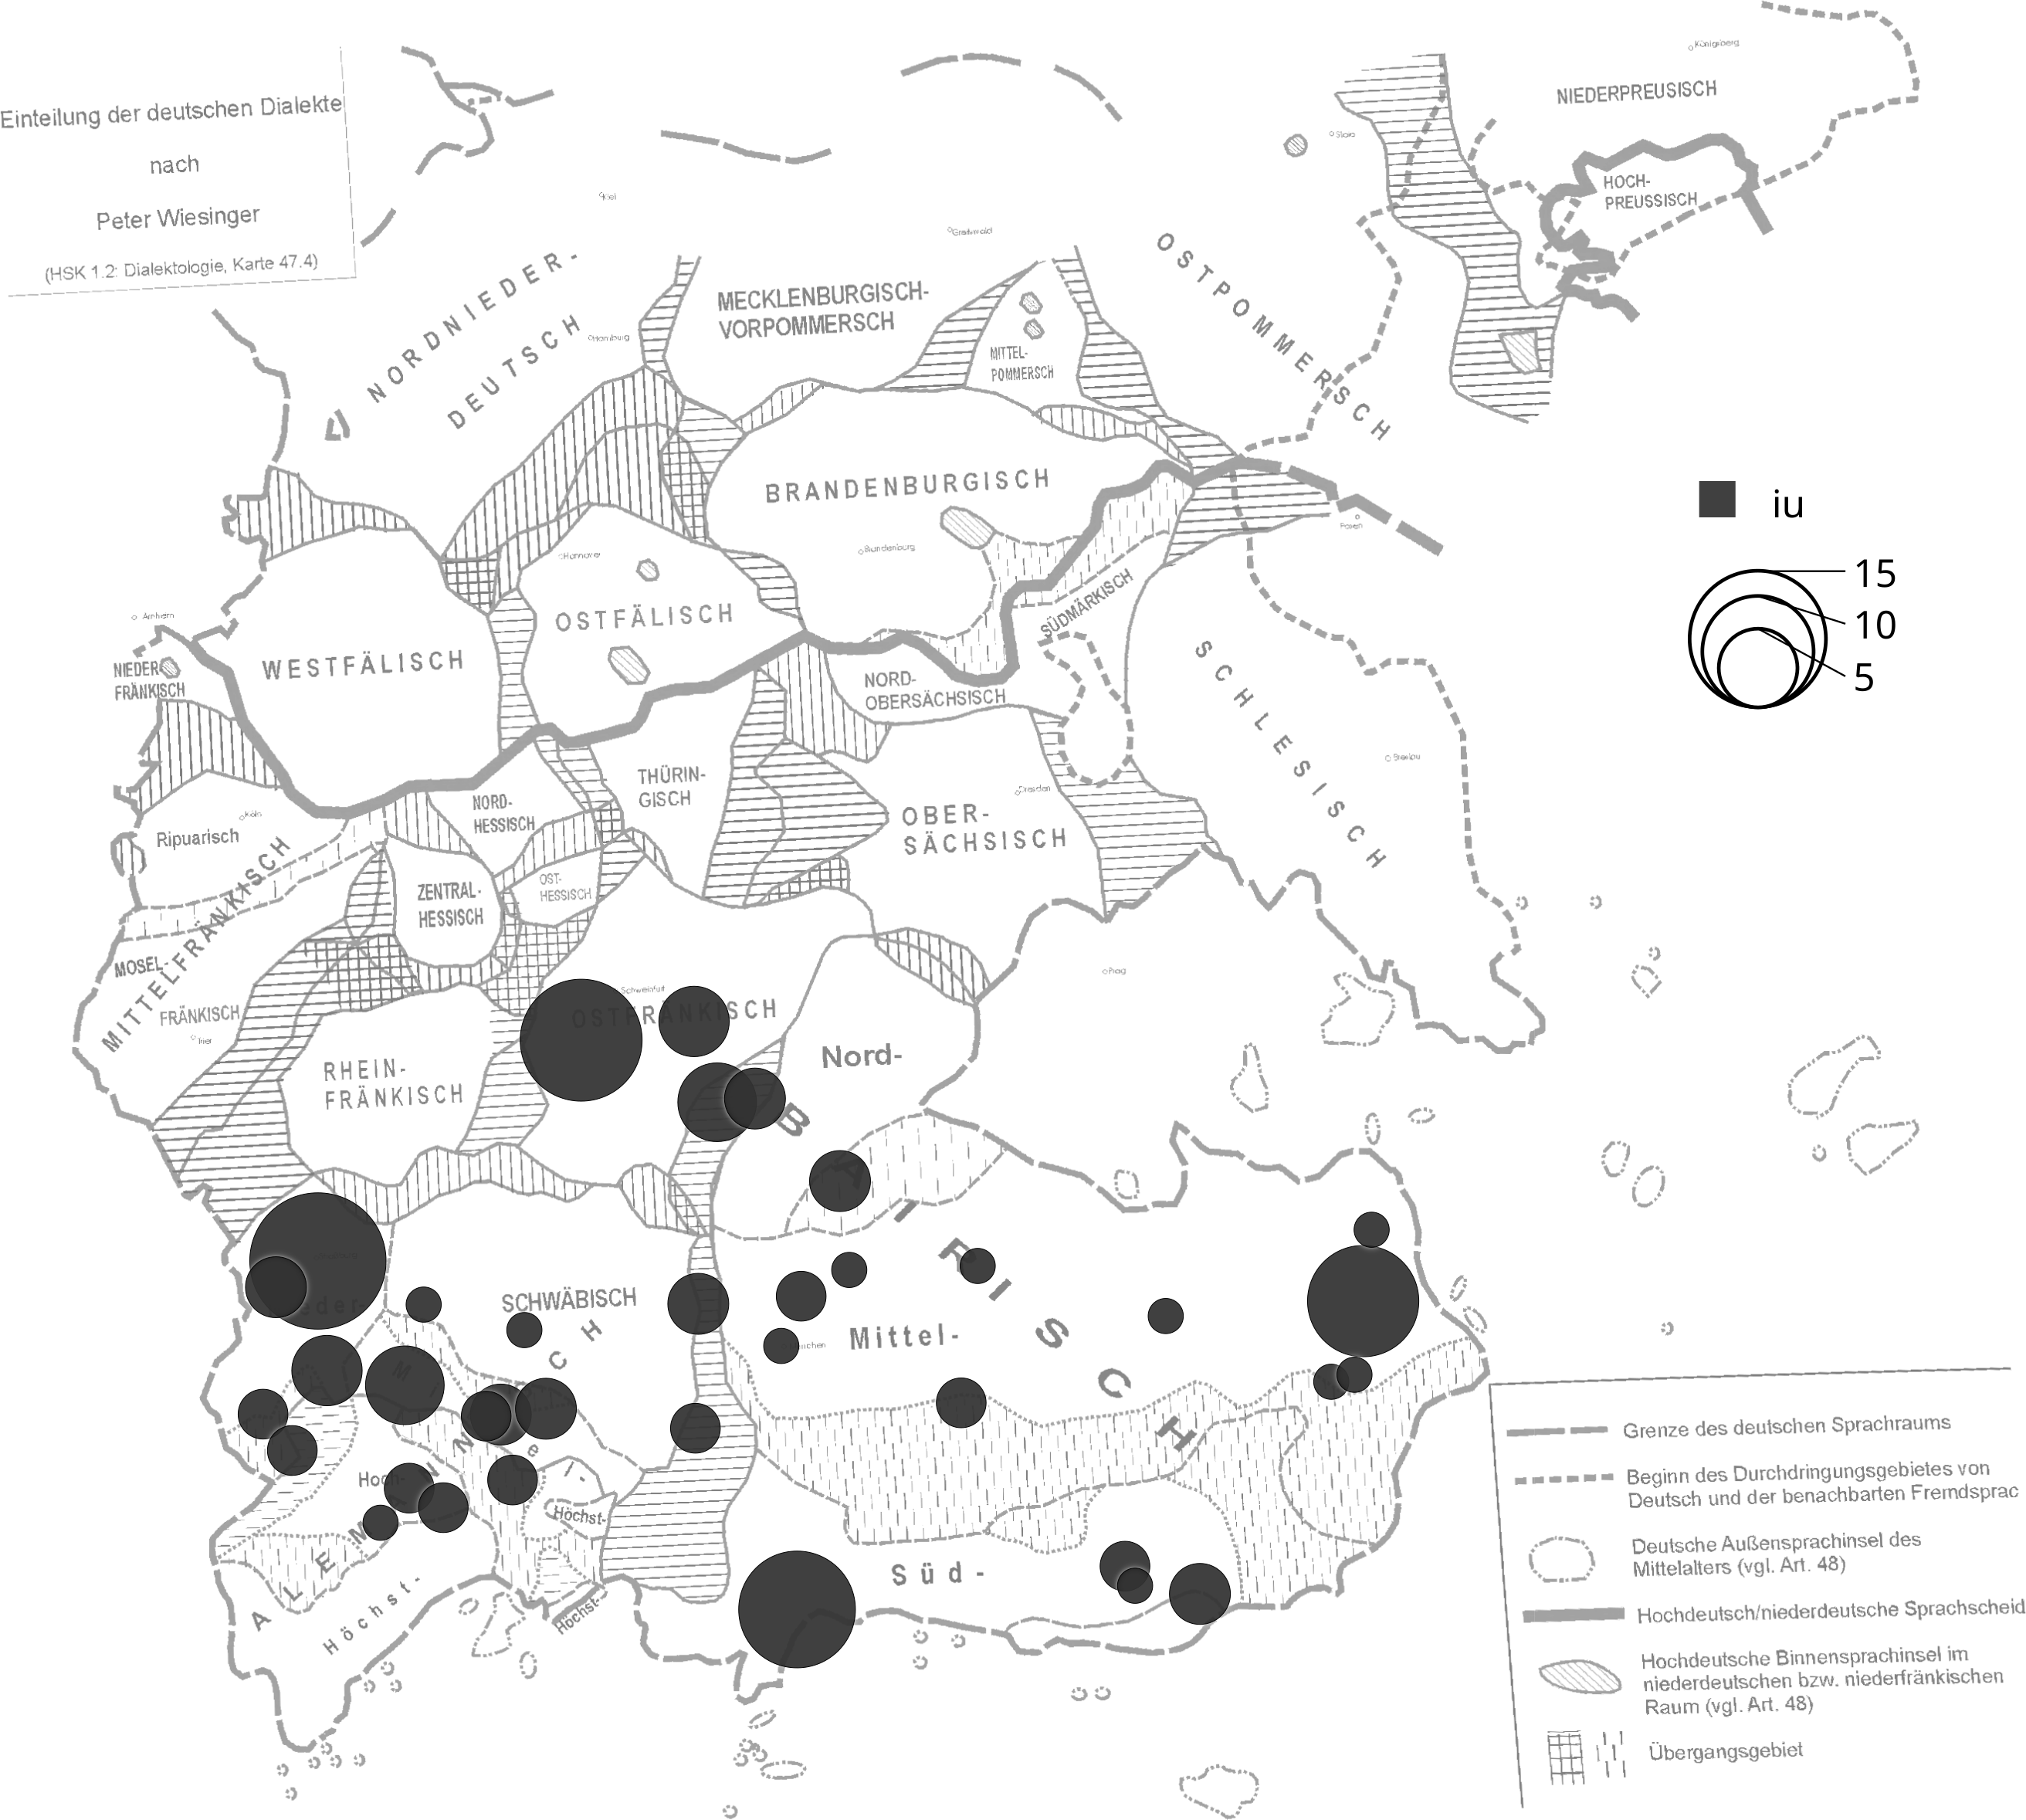
\includegraphics[
	width=\linewidth,
	keepaspectratio
]{./figures/2021-10-11_cao_beidiu-conj.png}
\caption{Geografische\is{Dialektgeografie}
	Distribution\is{Distribution!geografische} der Form \norm{bėidiu} in
	\norm{bėide \dots\ unde} `sowohl \dots\ als auch' (Hintergrundkarte:
	\cite{wiesinger1983:rede})}
\label{fig:cao_beideconj_geo_2}
\end{figure}

Darüber hinaus gibt \citet{gjelsten1980} zu bedenken, dass es
uneindeutige\is{Ambiguität} Fälle von \norm{bėide \dots\ unde} gibt, die man
\blockcquote[187]{gjelsten1980}{als appositive\is{Apposition} Konstruktionen
bewerten \textins{kann}, weil zwischen Pronomen und kopulativer Fügung
(\isi{Genus}-)Kongruenz besteht, oder als konjunktionale Konstruktionen, weil
die Pronominalform als erstarrte konjunktionale
Konstituente\is{Konstituentenstruktur} interpretierbar ist}.

Bei der Untersuchung haben sich im exzerpierten Material aber keine Muster
gezeigt, die eindeutig darauf hindeuten, dass bei der Annotation der
exzerpierten Belege regelmäßig Apposition\is{Apposition} und Konjunktion
verwechselt worden wären. Daneben liegen allerdings die zwei Belege in
\REF{ex:kczbeidenundesynt1} aus der \KC{}-Handschrift Z vor, in denen
\norm{bėide} eindeutig als Dativ flektiert erscheint.

\begin{exe}
\ex \label{ex:kczbeidenundesynt1}
\begin{xlist}
	\ex \label{ex:kczbeidenundesynt1_1}
		\gll Baiden man vnd wib \\
			beide-\textsc{dat.pl\subMF.st} Mann[\textsc{dat.sg.\MascM}] und
				Frau[\textsc{dat.sg.\NeutF}] \\
	\sn \gll Gebott er allen an den lyb \\
			gebot er all-\textsc{dat.pl\subMF.st} an den Leib \\
		\trans `Beiden, Mann und Frau, gebot er bei ihrem Leben'
			(%
				Z:~10va,9--10; vgl.~abweichend
				% C1:~3va,19--20; % beidev man vnd weip.
				% K:~3va,22--23; abweichend % [da]rzuͦ man vnd(e) wip
				% A1:~3va,1--2; % bediu wip unt man.
				% M:~5va,16--17; % Baidív wip vnd man.
				% H:~3vb,10--12; % Bede und(e) man.
				% B1:~3vc,51--53; % Baideu weip vnde man
				% VB:~3vb,5--7; % Beidiv wip vnd man
				% P:~6ra,8--10; % beide wip vnd(e) man.
				\KC:~V.~619--621;
				\cite[92]{schroeder1895}%
			)

	\protectedex{
	\ex \label{ex:kczbeidenundesynt1_2}
		\gll Baiden man vnd wÿb \\
				beide-\textsc{dat.pl\subMF.st} Mann[\textsc{dat.sg.\MascM}] und
					Frau[\textsc{dat.sg.\NeutF}] \\
	\sn \gll Sol es gan an den lÿb \\
			soll es gehen an den Leib \\
		\trans `Beiden, Mann und Frau, soll es ans Leben gehen.'
			(%
				Z:~15ra,18--19; vgl.~abweichend
				% C1:~4vb,2; % baidev man vnd weip.
				% K:~4vb,33--34; zu % Baidu̍ man vnd(e) wip
				\KC:~V.~846--849;
				\cite[97]{schroeder1895}%
			)
	}
\end{xlist}
\end{exe}

Da im Plural eine Form vom Typ \norm{wīben} zu erwarten wäre, wurden die
Substantive\is{Substantiv} hier als generisch verwendete
Singulare\is{generischer Gebrauch} aufgefasst. Das kataphorische\is{Katapher}
\lit{Baiden} bezieht sich zusammenfassend auf die nachfolgenden Konjunkte. Weil
\norm{bėide} die Zweizahl in seiner Bedeutung definiert, ist es notwendig, dass
die beiden singularischen Konjunkte \norm{man} `Mann' und \norm{wīp} ihre
\isi{Index}-Merkmale zu einem Plural vereinigen, damit ein zusammenhängender
und wohlgeformter Ausdruck entsteht. Im Dat.~Pl.\ der starken
\isi{Adjektivdeklination} spielt \isi{Genus} keine Rolle, insofern kann diese
Kategorie hier vernachlässigt werden, ansonsten wäre jedoch mit \isi{Gender
Resolution} zu rechnen. Aufgrund der Apposition\is{Apposition} muss
\norm{bėide} genauso wie die Konjunkte im Dativ stehen. \lit{Baiden} verkörpert
also zusammen mit dem konkretisierenden \norm{man unde wīp} das indirekte
Objekt von \lit{gebott} `gebot' beziehungsweise \lit{sol} `soll'.

Im Rahmen der LFG\is{Lexical-functional Grammar} deuten
\citet{sadlernordlinger2006} appositive\is{Apposition} Strukturen als Variante
von Koordination ohne overte Konjunktion. Sie diskutieren dies anhand von
Beispielen aus verschiedenen australischen Sprachen, in denen Koordination von
NPs durch einfache Nebeneinanderstellung der Konjunkte erreicht wird. Darüber
hinaus werde Nebeneinanderstellung nicht nur für asyndetische Koordination von
NPs verwendet, sondern auch für eine Reihe anderer, \q{appositionsartiger}
Konstruktionen \autocite[440--441]{sadlernordlinger2006}. Für
den vorliegenden Fall ist lediglich wichtig, dass bei Koordination das
\isi{Index}-Merkmal der Konjunkte aufgelöst wird, bei Apposition hingegen nicht
\autocite[444]{sadlernordlinger2006}. Die Beispiele in
\REF{ex:kczbeidenundesynt1} lassen sich daher wie in
\figref{fig:kczbeidenundesynt2} dargestellt modellieren.

\begin{figure}
	\begin{forest} shorter edges, narrower nodes, align text
	[{\anno[\pass{\SObj{recip}}]{DP\mysn{beidenunde_DP}}}
		[{\anno[\updownelem]{QP}}
			[\anno{\xhead{Q}}
				[bėiden, name=beiden, minimum width=3em]
			]
		]
		[{\anno[\updownelem]{NP}}
			[{\anno[\updownelem]{\xhead{N}}}
				[man]
			]
			[Conj
				[unde]
			]
			[{\anno[\updownelem]{\xhead{N}}}
				[wīp]
			]
		]
	]
	%
	% Annotation des Knotens zu breit, als dass die AVM noch hinpasst
	\node at (beiden) [below=1ex] {
		\smaller[2]\upshape\tabcolsep=.5ex%
		\begin{tabular}[t]{@{} l l l @{}}
			\ups{gf~case} & \req & \textsc{dat} \\
			\ups{gf~num}  & \req & \textsc{pl} \\
		\end{tabular}%
	};
	%
	\node [avmcontainer=0ex, font=\footnotesize] {
		\avm{%
		\tikzmark{beidenunde_f}$f$: [
			conj	& \textit{appos} \\
			\mc{2}{l}{%
				\{
					$g_1$: [
						pred	& `beide'
					]~$i$, \smallskip \\
					%
					$g_2$: [
						conj	& \textit{g-und} \\
						\mc{2}{l}{%
							\{
								$h_1$: [
									pred	& `Mann' \\
									pers	& 3 \\
									num		& \textsc{sg} \\
									gend	& \textsc{m} \\
									sex		& \SM \\
									case	& \textsc{dat}
								],
								$h_2$: [
								 	pred	& `Frau' \\
								 	pers	& 3 \\
								 	num		& \textsc{sg} \\
								 	gend	& \textsc{n} \\
								 	sex		& \SF \\
								 	case	& \textsc{dat}
								]
							\}%
						} \smallskip \\
						%
						index	& [
							pers	& 3 \\
							gend	& \textsc{n} \\
							num		& \textsc{pl}
						]
					]~$i$
				\}%
		}\smallskip \\
		index	& [
				pers	& 3 \\
				gend	& \textsc{n} \\
				num		& \textsc{pl}
			] \\
		]}
	};
	\end{forest}
	\begin{tikzpicture}[remember picture, overlay]
	\draw [myarrow]
		([yshift=.5ex]{pic cs:beidenunde_DP})
		to [out=east, in=north west]
		([yshift=.5ex]{pic cs:beidenunde_f});
	\end{tikzpicture}
	\caption{Analyse des Satzfragments \norm{bėiden, man unde wīp} `beiden,
		Mann und Frau'}
	\label{fig:kczbeidenundesynt2}
\end{figure}

In der F-Struktur\is{funktionale Struktur} auf der rechten Seite werden die
Konjunkte \norm{man} `Mann' und \norm{wīp} `Frau' in $g_2$ mit ihren
grammatischen Eigenschaften einzeln als $h_1$ und $h_2$ aufgelistet. Sie bilden
zusammen einen neuen \isi{Index} $i$, der die aufgelösten
Personenmerkmale\is{Personenmerkmal} enthält%
% (%
% 	\{\SM\} $\cap$ \{\SF\} = \{\textsc{~}\} $\Rightarrow$ \textsc{n};
% 	\{\textsc{sg}\} $\cup$ \{\textsc{sg}\} $\Rightarrow$ \textsc{pl}%
% )
. Sodann bildet $g_1$ mit $g_2$ eine Apposition\is{Apposition} in $f$, wobei
das Pronomen \norm{bėiden} in $g_2$ mit $g_1$ koindiziert\is{Koindizierung}
ist. Beide Teile zusammengenommen haben ihrerseits ein \isi{Index}-Merkmal, das
hier allerdings dem \isi{Index} $i$ entspricht, da $g_1$ keine neuen
Informationen hinzufügt. In der C-Struktur\is{Konstituentenstruktur} auf der
linken Seite bilden \norm{man unde wīp} zusammen eine NP\is{Nominalphrase}, die
wiederum zusammen mit der QP\is{Quantorenphrase} \norm{bėiden} eine
DP\is{Determiniererphrase} bilden, die als indirektes Objekt dient.

\is{Konjunktion|)}
\is{Koordination|)}
